\PassOptionsToPackage{unicode=true}{hyperref} % options for packages loaded elsewhere
\PassOptionsToPackage{hyphens}{url}
\PassOptionsToPackage{dvipsnames,svgnames*,x11names*}{xcolor}
%
\documentclass[french]{article}
\usepackage{lmodern}
\usepackage{amssymb,amsmath}
\usepackage{ifxetex,ifluatex}
\usepackage{fixltx2e} % provides \textsubscript
\ifnum 0\ifxetex 1\fi\ifluatex 1\fi=0 % if pdftex
  \usepackage[T1]{fontenc}
  \usepackage[utf8]{inputenc}
  \usepackage{textcomp} % provides euro and other symbols
\else % if luatex or xelatex
  \usepackage{unicode-math}
  \defaultfontfeatures{Ligatures=TeX,Scale=MatchLowercase}
\fi
% use upquote if available, for straight quotes in verbatim environments
\IfFileExists{upquote.sty}{\usepackage{upquote}}{}
% use microtype if available
\IfFileExists{microtype.sty}{%
\usepackage[]{microtype}
\UseMicrotypeSet[protrusion]{basicmath} % disable protrusion for tt fonts
}{}
\IfFileExists{parskip.sty}{%
\usepackage{parskip}
}{% else
\setlength{\parindent}{0pt}
\setlength{\parskip}{6pt plus 2pt minus 1pt}
}
\usepackage{xcolor}
\usepackage{hyperref}
\hypersetup{
            pdftitle={Projet de Séries Temporelles},
            pdfauthor={Kim Antunez et Alain Quartier-la-Tente},
            colorlinks=true,
            linkcolor=Maroon,
            filecolor=Maroon,
            citecolor=Blue,
            urlcolor=blue,
            breaklinks=true}
\urlstyle{same}  % don't use monospace font for urls
\usepackage[margin=0.95in]{geometry}
\usepackage{color}
\usepackage{fancyvrb}
\newcommand{\VerbBar}{|}
\newcommand{\VERB}{\Verb[commandchars=\\\{\}]}
\DefineVerbatimEnvironment{Highlighting}{Verbatim}{commandchars=\\\{\}}
% Add ',fontsize=\small' for more characters per line
\usepackage{framed}
\definecolor{shadecolor}{RGB}{248,248,248}
\newenvironment{Shaded}{\begin{snugshade}}{\end{snugshade}}
\newcommand{\AlertTok}[1]{\textcolor[rgb]{0.94,0.16,0.16}{#1}}
\newcommand{\AnnotationTok}[1]{\textcolor[rgb]{0.56,0.35,0.01}{\textbf{\textit{#1}}}}
\newcommand{\AttributeTok}[1]{\textcolor[rgb]{0.77,0.63,0.00}{#1}}
\newcommand{\BaseNTok}[1]{\textcolor[rgb]{0.00,0.00,0.81}{#1}}
\newcommand{\BuiltInTok}[1]{#1}
\newcommand{\CharTok}[1]{\textcolor[rgb]{0.31,0.60,0.02}{#1}}
\newcommand{\CommentTok}[1]{\textcolor[rgb]{0.56,0.35,0.01}{\textit{#1}}}
\newcommand{\CommentVarTok}[1]{\textcolor[rgb]{0.56,0.35,0.01}{\textbf{\textit{#1}}}}
\newcommand{\ConstantTok}[1]{\textcolor[rgb]{0.00,0.00,0.00}{#1}}
\newcommand{\ControlFlowTok}[1]{\textcolor[rgb]{0.13,0.29,0.53}{\textbf{#1}}}
\newcommand{\DataTypeTok}[1]{\textcolor[rgb]{0.13,0.29,0.53}{#1}}
\newcommand{\DecValTok}[1]{\textcolor[rgb]{0.00,0.00,0.81}{#1}}
\newcommand{\DocumentationTok}[1]{\textcolor[rgb]{0.56,0.35,0.01}{\textbf{\textit{#1}}}}
\newcommand{\ErrorTok}[1]{\textcolor[rgb]{0.64,0.00,0.00}{\textbf{#1}}}
\newcommand{\ExtensionTok}[1]{#1}
\newcommand{\FloatTok}[1]{\textcolor[rgb]{0.00,0.00,0.81}{#1}}
\newcommand{\FunctionTok}[1]{\textcolor[rgb]{0.00,0.00,0.00}{#1}}
\newcommand{\ImportTok}[1]{#1}
\newcommand{\InformationTok}[1]{\textcolor[rgb]{0.56,0.35,0.01}{\textbf{\textit{#1}}}}
\newcommand{\KeywordTok}[1]{\textcolor[rgb]{0.13,0.29,0.53}{\textbf{#1}}}
\newcommand{\NormalTok}[1]{#1}
\newcommand{\OperatorTok}[1]{\textcolor[rgb]{0.81,0.36,0.00}{\textbf{#1}}}
\newcommand{\OtherTok}[1]{\textcolor[rgb]{0.56,0.35,0.01}{#1}}
\newcommand{\PreprocessorTok}[1]{\textcolor[rgb]{0.56,0.35,0.01}{\textit{#1}}}
\newcommand{\RegionMarkerTok}[1]{#1}
\newcommand{\SpecialCharTok}[1]{\textcolor[rgb]{0.00,0.00,0.00}{#1}}
\newcommand{\SpecialStringTok}[1]{\textcolor[rgb]{0.31,0.60,0.02}{#1}}
\newcommand{\StringTok}[1]{\textcolor[rgb]{0.31,0.60,0.02}{#1}}
\newcommand{\VariableTok}[1]{\textcolor[rgb]{0.00,0.00,0.00}{#1}}
\newcommand{\VerbatimStringTok}[1]{\textcolor[rgb]{0.31,0.60,0.02}{#1}}
\newcommand{\WarningTok}[1]{\textcolor[rgb]{0.56,0.35,0.01}{\textbf{\textit{#1}}}}
\usepackage{longtable,booktabs}
% Fix footnotes in tables (requires footnote package)
\IfFileExists{footnote.sty}{\usepackage{footnote}\makesavenoteenv{longtable}}{}
\usepackage{graphicx,grffile}
\makeatletter
\def\maxwidth{\ifdim\Gin@nat@width>\linewidth\linewidth\else\Gin@nat@width\fi}
\def\maxheight{\ifdim\Gin@nat@height>\textheight\textheight\else\Gin@nat@height\fi}
\makeatother
% Scale images if necessary, so that they will not overflow the page
% margins by default, and it is still possible to overwrite the defaults
% using explicit options in \includegraphics[width, height, ...]{}
\setkeys{Gin}{width=\maxwidth,height=\maxheight,keepaspectratio}
\setlength{\emergencystretch}{3em}  % prevent overfull lines
\providecommand{\tightlist}{%
  \setlength{\itemsep}{0pt}\setlength{\parskip}{0pt}}
\setcounter{secnumdepth}{5}
% Redefines (sub)paragraphs to behave more like sections
\ifx\paragraph\undefined\else
\let\oldparagraph\paragraph
\renewcommand{\paragraph}[1]{\oldparagraph{#1}\mbox{}}
\fi
\ifx\subparagraph\undefined\else
\let\oldsubparagraph\subparagraph
\renewcommand{\subparagraph}[1]{\oldsubparagraph{#1}\mbox{}}
\fi

% set default figure placement to htbp
\makeatletter
\def\fps@figure{htbp}
\makeatother

\usepackage[french]{babel}
\usepackage{fontawesome5}
\usepackage{multicol}
\DeclareMathOperator{\Cov}{Cov}
\usepackage{mathtools}
\usepackage{caption}
\usepackage{xspace}
\usepackage{textpos}
\usepackage{booktabs}
\usepackage{longtable}
\usepackage{array}
\usepackage{multirow}
\usepackage{wrapfig}
\usepackage{float}
\usepackage{colortbl}
\usepackage{pdflscape}
\usepackage{tabu}
\usepackage{threeparttable}
\usepackage{threeparttablex}
\usepackage[normalem]{ulem}
\usepackage{makecell}
\usepackage{xcolor}

\title{Projet de Séries Temporelles}
\author{Kim Antunez et Alain Quartier-la-Tente}
\date{19/05/2020}

\begin{document}
\maketitle

{
\hypersetup{linkcolor=}
\setcounter{tocdepth}{3}
\tableofcontents
}
\begin{textblock*}{\textwidth}(0cm,-14.cm)
\begin{center}

\includegraphics[height=2cm]{img/LOGO-ENSAE-avatar.png}
\end{center}
\end{textblock*}

\thispagestyle{empty}
\newpage\setcounter{page}{1}

\hypertarget{partie-1-les-donnuxe9es}{%
\section{Partie 1 : Les données}\label{partie-1-les-donnuxe9es}}

\hypertarget{question-1-description-de-la-suxe9rie-choisie}{%
\subsection{Question 1 : description de la série choisie}\label{question-1-description-de-la-suxe9rie-choisie}}

Pour ce projet, travaillons sur la série d'indice de production industrielle (IPI) dans l'industrie automobile (identifiant : \href{https://bdm.insee.fr/series/sdmx/data/SERIES_BDM/010537940}{010537940}).
Il s'agit d'une série au niveau A64 de la nomenclature d'activités française révision 2 (NAF rév. 2, division 29), poste CL1.
L'industrie automobile concerne aussi bien la production des constructeurs de voitures particulières, de véhicules de loisir, de véhicules utilitaires que les équipementiers spécialisés, les carrossiers, les assembleurs ou les prestataires de services d'aménagement de véhicules automobiles.
Cette production intègre donc la filière complète, y compris moteurs et organes mécaniques en amont, dès lors qu'ils sont principalement destinés à des véhicules automobiles (à l'exception des parties de moteur).

Il s'agit d'un indice de Laspeyres\footnote{Les indices de Laspeyres et de Paasche permettent de synthétiser en un indice unique un certain nombre d'indices. L'indice de Laspeyres, le plus célèbre est l'IPC (indice des prix à la consommation).}, en base 2015, chaîné avec des pondérations annuelles (les pondérations correspondant aux valeurs ajoutées des branches associées).
L'IPI dans l'industrie automobile est calculé à partir de l'enquête mensuelle de branche, par agrégation de séries ``élémentaires'' estimées en volume\footnote{La série d'IPI dans l'industrie automobile ne tient donc pas compte des variations de prix.}, calculées à un niveau plus fin.

Les séries de l'IPI sont corrigées des variations saisonnières et des jours ouvrables (CVS-CJO) à partir de la méthode X13-ARIMA.
La désaisonnalisation est réalisée de manière indirecte : elle est effectuée à un niveau fin et les agrégats CVS-CJO sont ensuite calculés directement à partir de ces séries en agrégeant les séries CVS-CJO.
Cette désaisonnalisation est réalisée par sous-périodes pour prendre en compte le fait que la structure économique des séries a beaucoup évolué en 30 ans, et donc qu'il serait peut pertinent d'appliquer un seul modèle de désaisonnalisation sur l'ensemble de la période.
Ainsi, les modèles utilisés pour la désaisonnalisation commencent en 2005 et ces modèles sont utilisées pour estimer les séries CVS-CJO à partir de 2012.

Les séries CVS-CJO avant et après 2012 n'étant pas évaluées sur les mêmes modèles, l'idéal serait d'étudier notre série après janvier 2012 pour éviter des ruptures liées à ce changement de modèle. En revanche, cela laisserait une faible profondeur temporelle risquant de fragiliser l'estimation de nos modèles ARIMA.
C'est pourquoi nous allons étudier la série d'IPI dans l'industrie automobile entre \textbf{janvier 2010 et décembre 2019}\footnote{Lorsque nous avons commencé ce projet, l'IPI était disponible jusqu'en février 2020.
  En revanche, les derniers points étant souvent sujets à révisions, nous avons préféré ne pas prendre en compte les points de janvier et février 2020.}, c'est-à-dire sur \textbf{120 observations}.

Nous n'effectuons pas ici de correction de point atypique ou de transformation logarithmique.

\hypertarget{questions-2-et-3-transformation-de-la-suxe9rie}{%
\subsection{Questions 2 et 3 : transformation de la série}\label{questions-2-et-3-transformation-de-la-suxe9rie}}

\begin{figure}

{\centering 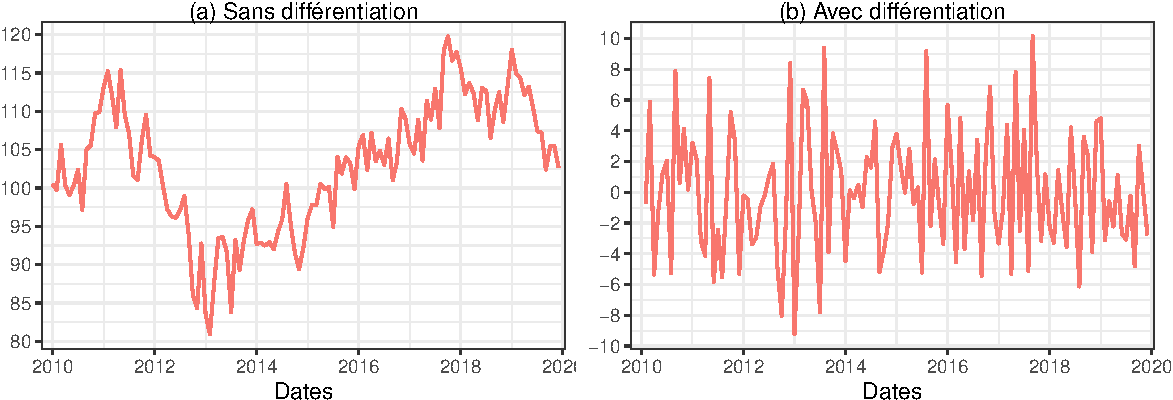
\includegraphics{img/rmd-compGraph-1} 

}

\caption{IPI dans l'automobile (CVS-CJO) sans et avec différentiation.}\label{fig:compGraph}
\end{figure}

Le graphique \ref{fig:compGraph}-(a) ne montre pas de tendance linéaire déterministe nette sur la période 2010-2020 : on observe plutôt une alternance entre des périodes à tendance croissante (2010-2011, 2013-2018) et à tendance décroissante (2011-2013 et 2018-2020).
La série de l'IPI dans l'automobile semble plutôt montrer une tendance stochastique : elle n'est sûrement \textbf{pas stationnaire}. Ceci est vérifié en faisant le test Dickey-Fuller augmenté (ADF) avec une constante non nulle et sans tendance : on ne rejette pas l'hypothèse de présence de racine unitaire au seuil de 5 \% (tableau \ref{tab:tabTestsInit}).
Ceci est également confirmé par le test de racine unitaire de Phillips-Perron, non rejeté au seuil de 5 \%, et par le test de stationnarité\footnote{Ici, l'hypothèse alternative est la non-stationnarité de la série} de Kwiatkowski-Phillips-Schmidt-Shin (KPSS), rejeté au seuil de 5 \%. Nous \textbf{différencions} donc la série.

\begin{table}[!h]

\caption{\label{tab:tabTestsInit}Tests de racine unitaire et de stationnarité sur la série d'IPI dans l'automobile.}
\centering
\begin{threeparttable}
\begin{tabular}[t]{lccc}
\toprule
Test & Statistique & p-valeur & \\
\midrule
Dickey-Fuller augmenté \textsuperscript{a} & -1,678 & 0,434 & \\
Phillips-Perron & -2,578 & 0,336 & \\
KPSS & 0,892 & 0,010 & **\\
\bottomrule
\end{tabular}
\begin{tablenotes}
\item \hspace{-0.4cm}\textbf{Signif. codes: }0 `***' 0.001 `**' 0.01 `*' 0.05 `.' 0.1 ` ' 1
\item[a] Le test ADF a été fait en rajoutant 2 retards. De cette façon les résidus utilisés dans ce test sont bien indépendants et le test ADF est bien interprétable
\end{tablenotes}
\end{threeparttable}
\end{table}

D'après le graphique \ref{fig:compGraph}-(b), la série différenciée semble \textbf{stationnaire}.
Cette hypothèse est confirmée par le test de Dickey-Fuller augmenté, effectué avec une constante nulle et sans tendance, le test de Phillips-Perron et le test KPSS (tableau \ref{tab:tabTestsDiff}).

\begin{table}[!h]

\caption{\label{tab:tabTestsDiff}Tests de racine unitaire et de stationnarité sur la série différenciée d'IPI dans l'automobile.}
\centering
\begin{threeparttable}
\begin{tabular}[t]{lccc}
\toprule
Test & Statistique & p-valeur & \\
\midrule
Dickey-Fuller augmenté \textsuperscript{a} & -10,261 & 0,010 & **\\
Phillips-Perron & -15,132 & 0,010 & **\\
KPSS & 0,074 & 0,100 & .\\
\bottomrule
\end{tabular}
\begin{tablenotes}
\item \hspace{-0.4cm}\textbf{Signif. codes: }0 `***' 0.001 `**' 0.01 `*' 0.05 `.' 0.1 ` ' 1
\item[a] Le test ADF a été fait en rajoutant 1 retard. De cette façon les résidus utilisés dans ce test sont bien indépendants et le test ADF est bien interprétable
\end{tablenotes}
\end{threeparttable}
\end{table}

\hypertarget{partie-2-moduxe8les-arima}{%
\section{Partie 2 : Modèles ARIMA}\label{partie-2-moduxe8les-arima}}

Afin de déterminer les ordres maximaux, \(p_{max}\) et \(q_{max}\), du modèle \(ARMA(p,q)\) suivi par la série différenciée de l'IPI dans l'automobile, nous analysons les autocorrélogrammes et les autocorrélogrammes partiels (graphique~\ref{fig:acfPacf}).
À partir de retard 2 (inclus), aucun autocorrélogramme est significatif à 5 \% : on en déduit que \(p_{max} = 1\).
À partir de retard 2 (inclus), aucun autocorrélogramme partiel est significatif à 5 \%: on en déduit que \(q_{max} = 1\).\\
Ainsi, pour savoir quel(s) modèle(s) retenir, nous allons tester tous les modèles \(ARMA(p,q)\) tels que \(p\leq 1\) et \(q\leq 1\).

\begin{figure}

{\centering 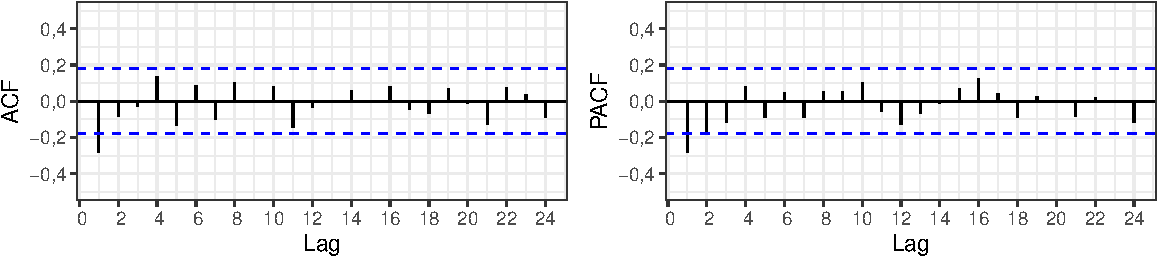
\includegraphics{img/rmd-acfPacf-1} 

}

\caption{Autocorrélogrammes (ACF) et autocorrélogrammes partiels (PACF) pour la série différenciée de l'IPI dans l'automobile.}\label{fig:acfPacf}
\end{figure}

Quatre modèles ARMA ont donc été testés\footnote{Ils ont été estimés sans constante.} afin de s'assurer de l'indépendance des résidus (tableau \ref{tab:tablbtest}) et, si c'est bien le cas, de la significativité des coefficients associés aux ordres maximaux des parties AR et MA des modèles (tableau \ref{tab:tabcoefs}) :

\begin{itemize}
\item \emph{ARMA(0,0)} : les résidus de ce modèle ne sont pas indépendants \faArrowCircleRight{} \textbf{modèle non retenu}

\item \emph{ARMA(1,0)} : les résidus de ce modèle ne sont pas indépendants \faArrowCircleRight{} \textbf{modèle non retenu}

\item \emph{ARMA(0,1)} : les résidus de ce modèle sont indépendants et le coefficient associé au MA(1) est significatif \faArrowCircleRight{} \textbf{modèle retenu}

\item \emph{ARMA(1,1)} : les résidus de ce modèle sont indépendants (tableau mais le coefficient associé au AR(1) n'est significatif \faArrowCircleRight{} \textbf{modèle non retenu}
\end{itemize}

Finalement, seul le modèle ARMA(0,1) est valide sur la série différenciée. Sur la série non différenciée de l'IPI automobile, on retient donc le modèle \textbf{ARIMA(0,1,1)} défini mathématiquement par :

\[
\Delta X_t = \varepsilon_t - \underset{(0,09)}{0,38}\;\varepsilon_{t-1}
\]
\(\varepsilon_t\) est bien un bruit blanc : les \((\varepsilon_t)_t\) sont indépendants (tableau \ref{tab:tablbtest}), homoscédastiques (tableau \ref{tab:tablb2test}) et suivent aussi une loi normale (tableau \ref{tab:tabjb}).

Parmi l'ensemble des modèles testés, l'ARIMA(0,1,1) est aussi le modèle qui minimise les critères d'information (tableau \ref{tab:aicbic}).

\begin{table}[!h]

\caption{\label{tab:aicbic}Critères d'information des modèles ARIMA sur l'IPI de l'automobile.}
\centering
\begin{tabular}[t]{lcccc}
\toprule
  & ARIMA(0,1,0) & ARIMA(1,1,0) & ARIMA(0,1,1) & ARIMA(1,1,1)\\
\midrule
AIC & 672,439 & 664,677 & 660,932 & 662,345\\
BIC & 675,219 & 670,235 & 666,490 & 670,683\\
\bottomrule
\end{tabular}
\end{table}

\hypertarget{partie-3-pruxe9visions}{%
\section{Partie 3 : Prévisions}\label{partie-3-pruxe9visions}}

\hypertarget{question-6-7-et-8-construction-dun-intervalle-de-confiance}{%
\subsection{Question 6, 7 et 8 : construction d'un intervalle de confiance}\label{question-6-7-et-8-construction-dun-intervalle-de-confiance}}

On cherche désormais à faire une prévision de \(X_t\) à l'horizon \(T+2\).
Notons \(\theta_1\) le coefficient associé à la partie MA de notre modèle ARMA(0,1,1), qu'on estime par \(\widehat\theta_1\simeq -0,38\) (tableau \ref{tab:tabcoefs}) en estimant le modèle entre janvier 2010 et décembre 2019. On a donc :
\[
\Delta X_T = \varepsilon_T + \theta_1\varepsilon_{T-1}
\iff 
X_T = X_{T-1} + \varepsilon_T + \theta_1\varepsilon_{T-1}
\quad\text{où}\quad
\varepsilon_t\overset{i.i.d}\sim\mathcal N(0,\sigma^2)
\]

En considérant \(\theta_1\) connu, les prévisions de \(X_{T+1}\) et \(X_{T+2}\) réalisées à l'instant \(T\), notées \(\widehat X_{T+1\vert T}\) et \(\widehat X_{T+2\vert T}\), vérifient l'équation :
\[
\begin{cases}
\widehat X_{T+1\vert T}= X_T + \theta_1\varepsilon_T \\
\widehat X_{T+2\vert T}=\widehat X_{T+1\vert T} =  X_T + \theta_1\varepsilon_T 
\end{cases}
\]
Les erreurs de prévision sont égales à :
\[
\begin{cases}
\widehat \varepsilon_{T+1\vert T} = X_{T+1} - \widehat X_{T+1\vert T}=
\varepsilon_{T+1}+(\theta_1-\theta_1)\varepsilon_T 
&= \varepsilon_{T+1}
\\
\widehat \varepsilon_{T+2\vert T} = X_{T+2} - \widehat X_{T+2\vert T}=
\varepsilon_{T+2}+(1+\theta_1)\varepsilon_{T+1}+(\theta_1-\theta_1)\varepsilon_T 
&=
\varepsilon_{T+2}+(1+\theta_1)\varepsilon_{T+1}
\end{cases}
\]
Les \(\varepsilon_t\) étant i.i.d., \(\widehat \varepsilon_{T+h\vert T} \overset{(H_0)}{\sim}\mathcal N(0,\sigma_h^2)\) avec \(\sigma_1^2=\sigma^2\) et \(\sigma_h^2=\sigma^2(1+(1+\theta_1)^2)\).
De plus, \(\Cov(\widehat \varepsilon_{T+1\vert T},\widehat \varepsilon_{T+2\vert T})=\sigma^2(1+\theta_1)\). Donc :
\[
\begin{pmatrix}
    \widehat \varepsilon_{T+1\vert T} \\ \widehat \varepsilon_{T+2\vert T}
\end{pmatrix} \sim
\mathcal N \left(
\begin{pmatrix}
    0 \\ 0
\end{pmatrix}\right.,
\underbrace{
\sigma^2 
\begin{pmatrix}
    1 & 1+\theta_1\\ 1+\theta_1 & 1+ (1+\theta_1)^2
\end{pmatrix}}_{\Sigma}\left.\mathclap{\phantom{\begin{pmatrix} 0\\0 \end{pmatrix}}}
\right)
\]
D'où :
\[
\begin{pmatrix}
    \widehat \varepsilon_{T+1\vert T} & \widehat \varepsilon_{T+2\vert T}
\end{pmatrix}
\Sigma^{-1}
\begin{pmatrix}
    \widehat \varepsilon_{T+1\vert T} \\ \widehat \varepsilon_{T+2\vert T}
\end{pmatrix}\sim{\chi}^2(2) 
\quad\text{avec}\quad
\Sigma^{-1} = 
\frac{1}{\sigma^2}
\begin{pmatrix}
     1+(1+\theta_1)^2 & - (1+\theta_1) \\ -(1+\theta_1) &1
\end{pmatrix}
\]
En notant \(q_{1- \alpha}\) le quantile \(1- \alpha\) d'une loi \({\chi}^2(2)\), une région de confiance de niveau \(\alpha\) pour \((X_{T+1},X_{T+2})\) est :
\begin{equation}
R_\alpha=\left\{ 
\begin{pmatrix}
    x \\ y
\end{pmatrix}\: :\:
(1+(1+\theta_1)^2)(x-\widehat X_{T+1\vert T})^2-2(1+\theta_1)(x-\widehat X_{T+1\vert T})(y-\widehat X_{T+2\vert T}) + (y-\widehat X_{T+2\vert T})^2\leq \sigma^2q_{1-\alpha} 
\right\}
\label{eq:icCourtTerme}
\end{equation}

Le problème est que \(\sigma_h\) et \(\theta_1\) sont ici inconnus.
On estime donc \(\theta_1\) par \(\widehat \theta_1\), qui est l'estimation que l'on fait à partir de nos données et \(\sigma\) par \(\widehat \sigma= \frac{1}{T-2}\sum_{t=2}^T\widehat\varepsilon_t^2\).
En remplaçant \(\sigma_h\) et \(\theta_1\) par leurs valeurs estimées, la région de confiance définis dans l'équation \eqref{eq:icCourtTerme} reste valide mais \textbf{asymptotiquement uniquement}.

{[}\emph{Question 6}{]} En somme, la région de confiance pour \((X_{T+1},X_{T+2})\) est une ellipse, dont le centre est \((X_T + \widehat\theta_1\varepsilon_T, X_T + \widehat\theta_1\varepsilon_T)\) et caractérisé par l'équation :

\begin{equation}
\begin{split}
R_{1-\alpha}=\left\{ 
\begin{pmatrix}
    x \\ y
\end{pmatrix}\: :\:\right.
&(1+(1+\widehat\theta_1)^2)( X_T + \widehat\theta_1\varepsilon_T-x)^2
-
2(1+\widehat\theta_1)(X_T + \widehat\theta_1\varepsilon_T-x)(X_T + \widehat\theta_1\varepsilon_T-y) \\
&+
(X_T + \widehat\theta_1\varepsilon_T-y)^2\leq \widehat\sigma^2q_{1-\alpha} 
\left.\right\}
\end{split}
\label{eq:icPrev}
\end{equation}

L'application numérique (\(\alpha = 0,05\), \(\widehat\theta_1\simeq -0,38\), \(X_T\simeq102,66\), \(\varepsilon_T\simeq-2,63\), \(\hat \sigma^2 \simeq 14,73\), \(q_{0,95} \simeq 5,99\)) donne :
\begin{equation}
R_{95\%}=\left\{ 
\begin{pmatrix}
    x \\ y
\end{pmatrix}\: :\:
0,016 x^2 - 0,014 \times x \times y + 0,011 y^2 - 1,798 x - 0,885 y + 139,044 = 1
\right\}
\label{eq:icApplique}
\end{equation}

{[}\emph{Question 7}{]} Pour obtenir cette région de confiance il faut :

\begin{itemize}
\tightlist
\item
  que le modèle suivit par notre série entre janvier 2010 et février 2020 soit bien un modèle ARIMA(0,1,1). Le modèle doit être en théorie parfaitement identifié (\(\sigma\) et \(\theta_1\) connus ou a minima que leurs estimateurs convergent vers leurs valeurs) ;
\item
  que les résidus de notre modèle ARIMA soient \textbf{indépendants, homoscédastiques et suivent une loi normale} : ce qui a bien été vérifié dans la partie précédente ;
\item
  que \(T\) soit grand (dans notre cas \(T=120\)).
\end{itemize}

{[}\emph{Question 8}{]} Le graphique \ref{fig:RegIC} présente la région de confiance au seuil 95 \%, les intervalles de confiance associés aux deux prévision (lorsqu'on les calcule de manière indépendante pour \(X_{T+1}\) et \(X_{T+2}\)), ainsi que les dernières valeurs publiées de l'IPI automobile de janvier et de février 2020.
On retrouve ce que l'on a montré par l'équation \eqref{eq:icPrev} : la même valeur est prédite pour \(X_{T+1}\) et \(X_{T+2}\).
Prédire les mêmes valeurs pour les deux dates paraît économiquement peu cohérent, mais cela reflète la dynamique du modèle ARIMA(0,1,1) :

\begin{itemize}
\item
  Puisqu'il y a aucun ordre autorégressif, \(\Delta X_t\) ne dépend pas des valeurs passées prises par \((\Delta X_{t'})_{t'\leq t-1}\).
\item
  Puisque l'ordre MA est égal à 1, il n'y a aucune influence du bruit à l'horizon supérieur ou égal à 2 : sans aucune information supplémentaire, la seule prévision possible pour \(\Delta X_{t+h}\), \(h\geq 2\), est une prévision nulle, et donc pour \(X_{t+h}\) la seule prévision possible est \(\widehat X_{t+1\vert t}\).
  Cette incertitude se traduit par une région de confiance très large\footnote{On prévoit une évolution mensuelle entre décembre 2019 et janvier 2020 comprise entre -6,8 \% et +8,7 \%, ce qui est très grand compte tenu de la volatilité de la série (l'écart-type de la série en évolution est de 4,1 et sa moyenne de 0,1).}.
\end{itemize}

La forme allongée et orientée à 45 degrés de la région de confiance reflète une certaine cohérence entre les prévisions de \(X_{T+1}\) et \(X_{T+2}\) (que l'on a pas quand on construit des intervalles de confiance de manière indépendante).
En effet, plus \(\widehat X_{T+1\vert T}\) est grand, plus les valeurs «~plausibles~» de \(\widehat X_{T+2\vert T}\) sont élevées.
Toutefois, le grand axe de l'ellipse n'est pas aligné à la première bissectrice : si \(\widehat X_{T+1\vert T}\) atteint sa plus grande valeur possible alors \(\widehat X_{T+2\vert T}<\widehat X_{T+1\vert T}\) (il y a dans ce cas un contrecoup économique).

\begin{figure}[htbp]
\begin{center}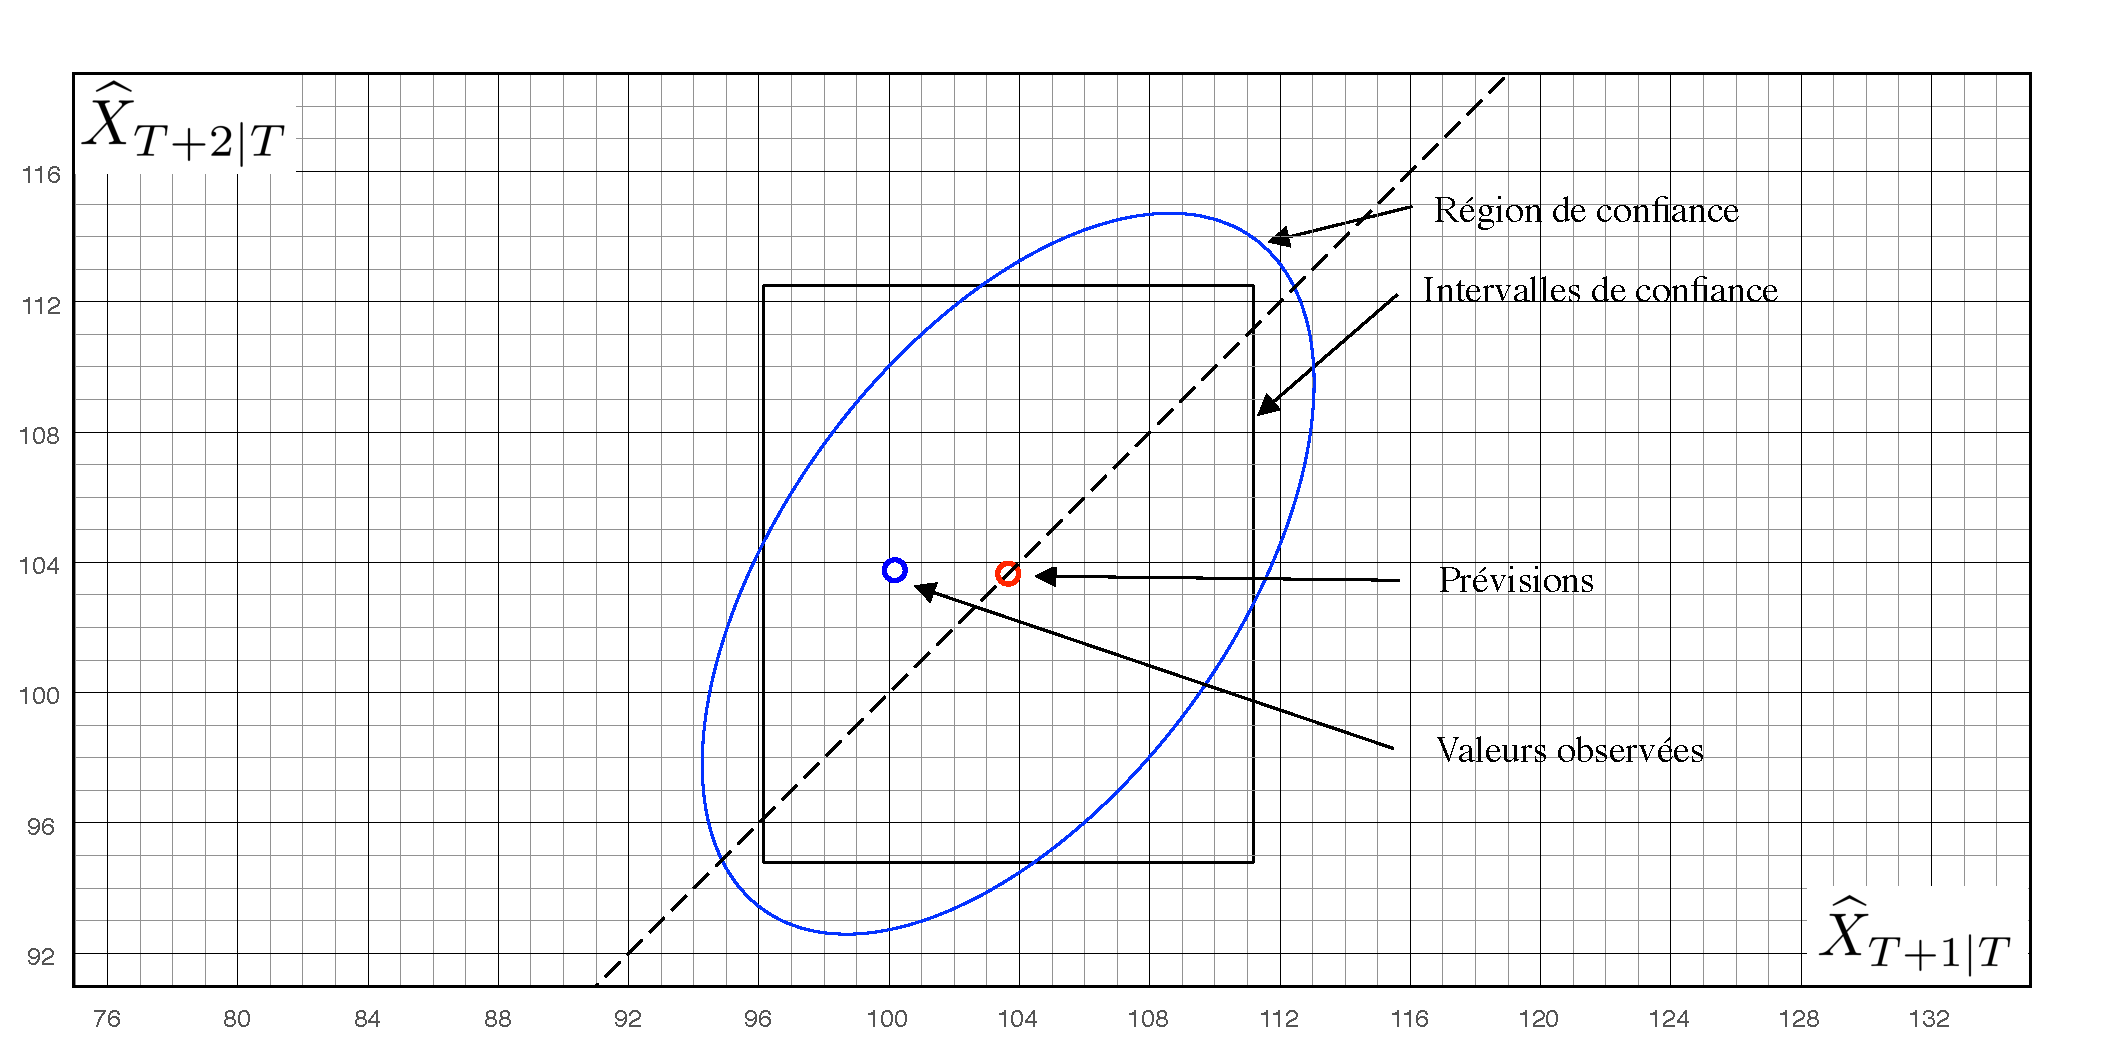
\includegraphics[width = 0.8\textwidth]{img/ellipse} \end{center}
\captionsetup{margin=0cm,format=hang,justification=justified}
\caption{Région de confiance pour la prévision de l'IPI automobile CVS-CJO pour janvier et février 2020 par un modèle ARIMA(0,1,1)}\label{fig:RegIC}
\end{figure}

\begin{figure}

{\centering 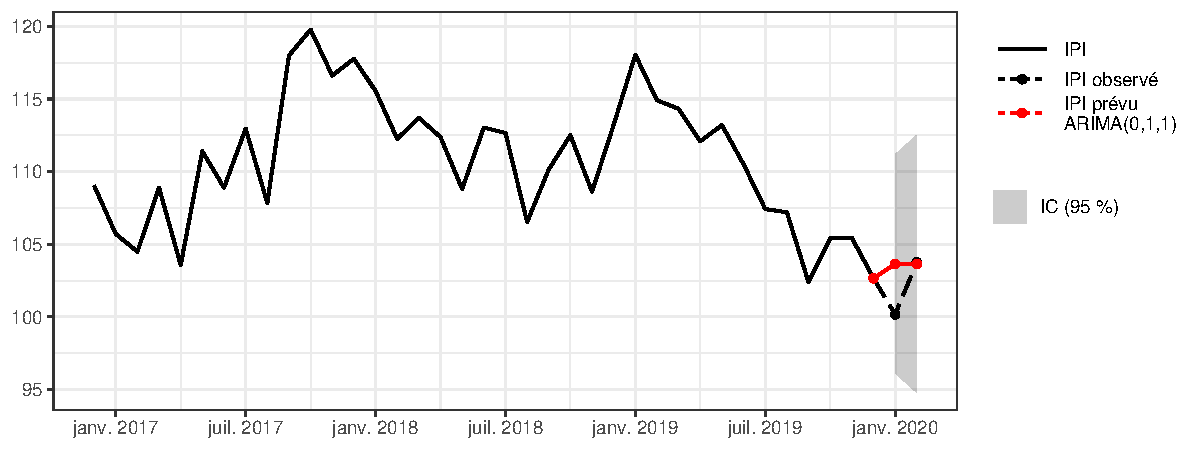
\includegraphics{img/rmd-prevIpi-1} 

}

\caption{Prévisions de l'IPI automobile CVS-CJO pour janvier et février 2020 par un modèle ARIMA(0,1,1).}\label{fig:prevIpi}
\end{figure}

\hypertarget{question-9-question-ouverte-sur-la-causalituxe9}{%
\subsection{Question 9 : question ouverte sur la causalité}\label{question-9-question-ouverte-sur-la-causalituxe9}}

Soit \(Y_t\) une série stationnaire disponible de \(t = 1\) à \(T\) telle que \(Y_{T+1}\) est disponible plus rapidement que \(X_{T+1}\).

\(Y_t\) cause\footnote{Cette notion de causalité n'est pas la même que celle utilisée en économétrie classique (une influence directe de \(Y_t\) sur \(X_t\)), cela signifie simplement ici que \(Y_t\) est utile pour prévoir \(X_t\).} instantanément \(X_t\) au sens de Granger (\(C_{X - Y}\)\footnote{La relation de causalité instantanée de Granger est symétrique : \(C_{X - Y} \iff C_{Y - X}\).}) si et seulement si pour tout \(t\), la valeur de \(Y_{t+1}\) permet d'améliorer la prévision de \(X_{t+1}\).
Ainsi, la causalité instantanée au sens de Granger est une condition suffisante pour que \(Y_{T+1}\) permette d'améliorer la prévision de \(X_{T+1}\).
Mathématiquement :

\[ \underbrace{\forall t \quad \widehat X_{t+1 \vert \{Y_u, X_u, u \le t \}  \cup \{Y_{t+1}\}}   \ne \widehat X_{t+1 \vert \{Y_u, X_u, u \le t \}}}_{C_{X - Y} \text{ }:\text{ } Y_t \textrm{ cause instantanément au sens de Granger } X_t} \overset{\text{en particulier}}{\Longrightarrow} \widehat X_{T+1 \vert \{Y_{1 \dots T},X_{1 \dots T}\} \cup \{Y_{T+1}\}} \ne \widehat X_{T+1 \vert \{Y_{1 \dots T},X_{1 \dots T}\}}\]

Cette définition de causalité instantanée est fondée sur les corrélations entre les erreurs.
En effet, si \((Y_t',X_t')'\) est bien \textbf{stationnaire} alors on a montré dans le cours que :

\[C_{X - Y} \iff Cov(\epsilon_{1t},\epsilon_{2t}) = 0 \quad \text{avec} \quad \begin{pmatrix} \epsilon_{1t}
\\\epsilon_{2t}\end{pmatrix} = \begin{pmatrix} Y_t - \widehat Y_{t \vert \{Y_u, X_u, u \le t-1 \}}
\\\ X_t - \widehat X_{t \vert \{Y_u, X_u, u \le t-1 \}}\end{pmatrix}\]

En prenant bien le soin de choisir \(X_t\) et \(Y_t\) de manière à ce que \((Y_t',X_t')'\) soit stationnaire, vérifier que \(Y_{T+1}\) permet d'améliorer la prévision de \(X_{T+1}\) revient alors à tester la condition suivante après avoir estimé les modèles correspondants à l'évolution de \(X_t\) et \(Y_t\) :

\[Cov( Y_{T+1} - \widehat Y_{T+1 \vert \{Y_{1 \dots T},X_{1 \dots T} \} }, X_{T+1} - \widehat X_{T+1 \vert \{Y_{1 \dots T},X_{1 \dots T} \} }) = 0\]
En notant \(X_t\) notre série de l'IPI de l'industrie automobile stationnarisée, il faudrait par exemple prendre pour \(Y_t\) des données susceptibles d'être disponibles avant \(X_t\) et feraient de bons candidats pour prévoir l'évolution de l'IPI dans l'industrie automobile :

\begin{itemize}
\item
  un IPI correspondant à une composante de la division « industrie automobile » (29)\footnote{Par exemple une des classes parmi la construction de véhicules automobiles (29.1), la fabrication de carrosseries et remorques (29.2) ou les équipements automobiles (29.3).} qu'il faudrait différencier autant de fois que nécessaire pour qu'elle soit bien stationnaire.
  Certaines composantes peuvent en effet disponibles être avant leur agrégat.
\item
  une série stationnaire issue d'une autre enquête qui donnerait de l'information sur la production de l'IPI de l'industrie automobile.
  Cela peut par exemple être le cas des résultats des enquêtes de conjoncture, de l'Insee ou de la Banque de France, auprès des entreprises de ce secteur.
  Dans ces enquêtes on demande en effet l'opinion des chefs d'entreprise sur l'évolution passée et future de leur production : ces informations sont qualitatives et sont donc connues bien avant les informations quantitatives demandées par l'enquête mensuelle de branche.
\end{itemize}

Il peut également exister des cas où \(Y_{T+1}\) permet d'améliorer la prévision de \(X_{T+1}\) mais sans que \(Y_t\) cause instantanément \(X_t\).\\
Prenons, par exemple, pour \(X_T\) la série stationnarisée de l'indice de production industrielle dans la cokéfaction-raffinage.
Cette série est très bruitée car en France la production de ce poste est concentrée en une dizaine de raffineries.
Ainsi, il est très difficile d'avoir une prévision précise de cette série qui sera très sensible, par exemple, à l'arrêt d'une raffinerie pendant quelques jours.
En revanche, si on dispose d'un indicateur \(Y_t\) du nombre de jours de fermeture dans le mois, cette série peut, dans certains cas, permettre d'améliorer de manière conséquente la prévision de \(X_t\).
C'est par exemple le cas pendant les périodes de grèves : l'analyse de l'évolution de la production pendant les grèves passées permet d'estimer l'effet moyen d'un jour de grève, et cela permet donc d'estimer l'évolution future de la production pendant les mouvements sociaux futurs.\\
Si en \(T+1\) il y a des grèves dans les raffineries, \(Y_{T+1}\) est connu bien avant \(X_{T+1}\) et permet d'améliorer la prévision de \(X_{T+1}\).\\
Puisque les fermetures de raffineries sont rares (elles sont ouvertes tous les jours de la semaine), pour la majorité des périodes \(t\), \(Y_t\) ne permet pas d'améliorer la prévision de \(X_t\) : elle ne cause donc a priori pas instantanément \(X_t\) au sens de Granger.

\newpage

\hypertarget{appendix-appendix}{%
\appendix}


\setcounter{page}{0}
\pagenumbering{roman}

\hypertarget{sec:qualRes}{%
\section{Tests supplémentaires sur la qualité des modèles}\label{sec:qualRes}}

\begin{table}[!h]

\caption{\label{tab:tablbtest}Tests de Ljung-Box sur les résidus (tests d'autocorrélation) des modèles ARIMA sur l'IPI de l'automobile.}
\centering
\resizebox{\linewidth}{!}{
\begin{threeparttable}
\begin{tabular}[t]{ccccccccccccc}
\toprule
\multicolumn{1}{c}{ } & \multicolumn{2}{c}{ARIMA(0,1,0)} & \multicolumn{1}{c}{ } & \multicolumn{2}{c}{ARIMA(1,1,0)} & \multicolumn{1}{c}{ } & \multicolumn{2}{c}{ARIMA(0,1,1)} & \multicolumn{1}{c}{ } & \multicolumn{2}{c}{ARIMA(1,1,1)} & \multicolumn{1}{c}{ } \\
\cmidrule(l{3pt}r{3pt}){2-3} \cmidrule(l{3pt}r{3pt}){5-6} \cmidrule(l{3pt}r{3pt}){8-9} \cmidrule(l{3pt}r{3pt}){11-12}
Retards & Statistique & p-valeur &  & Statistique & p-valeur &  & Statistique & p-valeur &  & Statistique & p-valeur & \\
\midrule
1 & 9,652 & 0,002 & ** &  &  &  &  &  &  &  &  & \\
2 & 10,473 & 0,005 & ** & 4,757 & 0,029 & * & 0,858 & 0,354 &  &  &  & \\
3 & 10,580 & 0,014 & * & 4,796 & 0,091 & . & 0,925 & 0,630 &  & 0,106 & 0,744 & \\
4 & 12,843 & 0,012 & * & 6,191 & 0,103 &  & 1,985 & 0,576 &  & 1,544 & 0,462 & \\
5 & 15,122 & 0,010 & ** & 7,239 & 0,124 &  & 3,024 & 0,554 &  & 2,606 & 0,456 & \\
\addlinespace
6 & 16,041 & 0,014 & * & 7,327 & 0,197 &  & 3,165 & 0,675 &  & 2,907 & 0,573 & \\
7 & 17,341 & 0,015 & * & 7,800 & 0,253 &  & 3,566 & 0,735 &  & 3,389 & 0,640 & \\
8 & 18,808 & 0,016 & * & 8,936 & 0,257 &  & 4,884 & 0,674 &  & 4,676 & 0,586 & \\
9 & 18,809 & 0,027 & * & 9,306 & 0,317 &  & 5,129 & 0,744 &  & 4,781 & 0,687 & \\
10 & 19,645 & 0,033 & * & 9,610 & 0,383 &  & 5,338 & 0,804 &  & 5,037 & 0,754 & \\
\addlinespace
11 & 22,433 & 0,021 & * & 12,895 & 0,230 &  & 8,684 & 0,562 &  & 8,103 & 0,524 & \\
12 & 22,609 & 0,031 & * & 13,822 & 0,243 &  & 9,649 & 0,562 &  & 8,787 & 0,552 & \\
13 & 22,610 & 0,047 & * & 13,838 & 0,311 &  & 9,649 & 0,647 &  & 8,787 & 0,642 & \\
14 & 23,078 & 0,059 & . & 14,496 & 0,340 &  & 10,455 & 0,656 &  & 9,497 & 0,660 & \\
15 & 23,082 & 0,082 & . & 14,860 & 0,388 &  & 11,003 & 0,686 &  & 9,871 & 0,704 & \\
\addlinespace
16 & 24,077 & 0,088 & . & 15,947 & 0,386 &  & 12,232 & 0,661 &  & 11,074 & 0,680 & \\
17 & 24,339 & 0,111 &  & 16,263 & 0,435 &  & 12,411 & 0,715 &  & 11,227 & 0,736 & \\
18 & 24,935 & 0,127 &  & 16,911 & 0,460 &  & 12,993 & 0,737 &  & 11,795 & 0,758 & \\
19 & 25,633 & 0,141 &  & 17,430 & 0,494 &  & 13,173 & 0,781 &  & 11,966 & 0,802 & \\
20 & 25,649 & 0,178 &  & 17,579 & 0,551 &  & 13,432 & 0,816 &  & 12,208 & 0,836 & \\
\addlinespace
21 & 28,080 & 0,138 &  & 20,078 & 0,453 &  & 15,782 & 0,730 &  & 14,643 & 0,745 & \\
22 & 28,992 & 0,145 &  & 20,694 & 0,478 &  & 16,064 & 0,766 &  & 14,878 & 0,783 & \\
23 & 29,209 & 0,173 &  & 20,920 & 0,526 &  & 16,146 & 0,809 &  & 14,914 & 0,827 & \\
24 & 30,464 & 0,170 &  & 21,907 & 0,526 &  & 17,136 & 0,803 &  & 16,104 & 0,811 & \\
\bottomrule
\end{tabular}
\begin{tablenotes}
\item \hspace{-0.4cm}\textbf{Signif. codes: }0 `***' 0.001 `**' 0.01 `*' 0.05 `.' 0.1 ` ' 1
\item L’hypothèse (H0) d'indépendance des résidus n’est pas rejetée à 5 \% pour le modèle retenu ARIMA(0,1,1).
\end{tablenotes}
\end{threeparttable}}
\end{table}

\begin{table}[!h]

\caption{\label{tab:tabcoefs}Estimation des coefficients associés aux modèles ARIMA sur l'IPI de l'automobile.}
\centering
\begin{threeparttable}
\begin{tabular}[t]{lcccccccc}
\toprule
\multicolumn{1}{c}{ } & \multicolumn{3}{c}{AR(1)} & \multicolumn{1}{c}{ } & \multicolumn{3}{c}{MA(1)} & \multicolumn{1}{c}{ } \\
\cmidrule(l{3pt}r{3pt}){2-4} \cmidrule(l{3pt}r{3pt}){6-8}
  & Coefficient & Écart-type & p-valeur &  & Coefficient & Écart-type & p-valeur & \\
\midrule
ARIMA(0,1,0) &  &  &  &  &  &  &  & \\
ARIMA(1,1,0) & -0,280 & 0,088 & 0,001 & ** &  &  &  & \\
ARIMA(0,1,1) &  &  &  &  & -0,377 & 0,091 & 0,000 & ***\\
ARIMA(1,1,1) & 0,165 & 0,214 & 0,439 &  & -0,515 & 0,183 & 0,005 & **\\
\bottomrule
\end{tabular}
\begin{tablenotes}
\item \hspace{-0.4cm}\textbf{Signif. codes: }0 `***' 0.001 `**' 0.01 `*' 0.05 `.' 0.1 ` ' 1
\end{tablenotes}
\end{threeparttable}
\end{table}

\begin{table}[!h]

\caption{\label{tab:tablb2test}Tests de Ljung-Box sur le carré des résidus (tests d'homoscédasticité) des modèles ARIMA sur l'IPI de l'automobile.}
\centering
\resizebox{\linewidth}{!}{
\begin{threeparttable}
\begin{tabular}[t]{ccccccccccccc}
\toprule
\multicolumn{1}{c}{ } & \multicolumn{2}{c}{ARIMA(0,1,0)} & \multicolumn{1}{c}{ } & \multicolumn{2}{c}{ARIMA(1,1,0)} & \multicolumn{1}{c}{ } & \multicolumn{2}{c}{ARIMA(0,1,1)} & \multicolumn{1}{c}{ } & \multicolumn{2}{c}{ARIMA(1,1,1)} & \multicolumn{1}{c}{ } \\
\cmidrule(l{3pt}r{3pt}){2-3} \cmidrule(l{3pt}r{3pt}){5-6} \cmidrule(l{3pt}r{3pt}){8-9} \cmidrule(l{3pt}r{3pt}){11-12}
Retards & Statistique & p-valeur &  & Statistique & p-valeur &  & Statistique & p-valeur &  & Statistique & p-valeur & \\
\midrule
1 & 2,832 & 0,092 & . &  &  &  &  &  &  &  &  & \\
2 & 2,843 & 0,241 &  & 2,917 & 0,088 & . & 2,032 & 0,154 &  &  &  & \\
3 & 2,860 & 0,414 &  & 3,844 & 0,146 &  & 3,569 & 0,168 &  & 3,140 & 0,076 & .\\
4 & 3,227 & 0,521 &  & 5,425 & 0,143 &  & 4,164 & 0,244 &  & 3,575 & 0,167 & \\
5 & 3,233 & 0,664 &  & 5,448 & 0,244 &  & 4,183 & 0,382 &  & 3,576 & 0,311 & \\
\addlinespace
6 & 3,262 & 0,775 &  & 7,479 & 0,187 &  & 6,916 & 0,227 &  & 5,513 & 0,239 & \\
7 & 3,263 & 0,860 &  & 7,836 & 0,250 &  & 7,515 & 0,276 &  & 6,127 & 0,294 & \\
8 & 3,270 & 0,916 &  & 8,294 & 0,307 &  & 7,781 & 0,352 &  & 6,290 & 0,392 & \\
9 & 3,772 & 0,926 &  & 8,613 & 0,376 &  & 7,787 & 0,455 &  & 6,314 & 0,504 & \\
10 & 3,797 & 0,956 &  & 8,727 & 0,463 &  & 7,838 & 0,551 &  & 6,605 & 0,580 & \\
\addlinespace
11 & 5,286 & 0,917 &  & 9,343 & 0,500 &  & 8,071 & 0,622 &  & 6,897 & 0,648 & \\
12 & 5,482 & 0,940 &  & 10,431 & 0,492 &  & 9,136 & 0,609 &  & 7,987 & 0,630 & \\
13 & 5,619 & 0,959 &  & 11,058 & 0,524 &  & 9,537 & 0,656 &  & 8,373 & 0,680 & \\
14 & 7,532 & 0,912 &  & 12,221 & 0,510 &  & 10,714 & 0,635 &  & 9,807 & 0,633 & \\
15 & 7,727 & 0,934 &  & 12,252 & 0,586 &  & 10,784 & 0,703 &  & 9,807 & 0,710 & \\
\addlinespace
16 & 7,760 & 0,956 &  & 12,256 & 0,660 &  & 10,802 & 0,766 &  & 9,823 & 0,775 & \\
17 & 7,866 & 0,969 &  & 12,268 & 0,725 &  & 10,968 & 0,811 &  & 9,890 & 0,827 & \\
18 & 11,403 & 0,876 &  & 12,791 & 0,750 &  & 11,573 & 0,825 &  & 11,468 & 0,780 & \\
19 & 11,440 & 0,908 &  & 12,791 & 0,804 &  & 11,788 & 0,858 &  & 11,709 & 0,817 & \\
20 & 12,066 & 0,914 &  & 13,115 & 0,833 &  & 12,156 & 0,879 &  & 12,086 & 0,843 & \\
\addlinespace
21 & 12,213 & 0,934 &  & 14,050 & 0,828 &  & 13,228 & 0,867 &  & 12,984 & 0,839 & \\
22 & 13,751 & 0,910 &  & 15,070 & 0,819 &  & 14,231 & 0,859 &  & 14,364 & 0,812 & \\
23 & 14,907 & 0,898 &  & 15,242 & 0,852 &  & 14,284 & 0,891 &  & 14,389 & 0,852 & \\
24 & 15,944 & 0,890 &  & 16,450 & 0,835 &  & 16,650 & 0,826 &  & 16,688 & 0,780 & \\
\bottomrule
\end{tabular}
\begin{tablenotes}
\item \hspace{-0.4cm}\textbf{Signif. codes: }0 `***' 0.001 `**' 0.01 `*' 0.05 `.' 0.1 ` ' 1
\item L’hypothèse (H0) d'indépendance des résidus n’est pas rejetée à 5 \% pour le modèle retenu ARIMA(0,1,1).
\end{tablenotes}
\end{threeparttable}}
\end{table}

\begin{table}[!h]

\caption{\label{tab:tabjb}Tests de Jarque-Bera de normalité des résidus des modèles ARIMA sur l'IPI de l'automobile.}
\centering
\begin{threeparttable}
\begin{tabular}[t]{lccc}
\toprule
  & Statistique & p-valeur & \\
\midrule
ARIMA(0,1,0) & 2,381 & 0,304 & \\
ARIMA(1,1,0) & 2,414 & 0,299 & \\
ARIMA(0,1,1) & 2,363 & 0,307 & \\
ARIMA(1,1,1) & 2,241 & 0,326 & \\
\bottomrule
\end{tabular}
\begin{tablenotes}
\item \hspace{-0.4cm}\textbf{Signif. codes: }0 `***' 0.001 `**' 0.01 `*' 0.05 `.' 0.1 ` ' 1
\item Le test de Jarque-Bera suppose que les résidus soient indépendants et homoscédastiques.
\item L’hypothèse (H0) de normalité des résidus n’est pas rejetée à 5 \% pour l’ensemble des modèles et en particulier pour le modèle retenu ARIMA(0,1,1).
\end{tablenotes}
\end{threeparttable}
\end{table}

\newpage

~
\newpage

\hypertarget{code}{%
\section{\texorpdfstring{Code \faRProject{}}{Code }}\label{code}}

L'ensemble du code a été écrit avec l'encodage UTF-8.

\hypertarget{fichier-0---creation-des-donnees.r}{%
\subsection{\texorpdfstring{Fichier \texttt{0\ -\ Creation\ des\ donnees.R}}{Fichier 0 - Creation des donnees.R}}\label{fichier-0---creation-des-donnees.r}}

Code utilisé pour télécharger les données : non utile pour la suite puisque les données sont jointes au projet.

\begin{Shaded}
\begin{Highlighting}[]
\CommentTok{# Codes pour télécharger les séries : }
\CommentTok{# il n'est pas nécessaire de le relancer puisqu'elles}
\CommentTok{# sont toutes dans le dossier data/}

\CommentTok{# devtools::install_github("aqlt/AQLTools")}
 \KeywordTok{library}\NormalTok{(AQLTools)}
 \KeywordTok{library}\NormalTok{(zoo)}
 
\CommentTok{# CL1 = automobile}

\NormalTok{ipi_cl1 <-}\StringTok{ }\NormalTok{AQLTools}\OperatorTok{::}\KeywordTok{lectureBDM}\NormalTok{(}\StringTok{"010537940"}\NormalTok{)}
\NormalTok{ipi_cl1_brut <-}\StringTok{ }\NormalTok{AQLTools}\OperatorTok{::}\KeywordTok{lectureBDM}\NormalTok{(}\StringTok{"010537939"}\NormalTok{)}
\NormalTok{data_b <-}\StringTok{ }\KeywordTok{ts.union}\NormalTok{(ipi_cl1, ipi_cl1_brut)}
\NormalTok{data_}\DecValTok{2010}\NormalTok{ <-}\StringTok{ }\KeywordTok{window}\NormalTok{(data_b,}
                  \DataTypeTok{start =} \KeywordTok{c}\NormalTok{(}\DecValTok{2010}\NormalTok{, }\DecValTok{1}\NormalTok{),}
                  \DataTypeTok{end =} \KeywordTok{c}\NormalTok{(}\DecValTok{2019}\NormalTok{,}\DecValTok{12}\NormalTok{))}

\KeywordTok{saveRDS}\NormalTok{(data_b,}
        \DataTypeTok{file =} \StringTok{"data/donnees_completes.RDS"}\NormalTok{)}
\KeywordTok{saveRDS}\NormalTok{(data_}\DecValTok{2010}\NormalTok{,}
        \DataTypeTok{file =} \StringTok{"data/donnees.RDS"}\NormalTok{)}

\CommentTok{# Exporter en CSV : non utile pour lancer les programmes mais demandé par les consignes}
\KeywordTok{write.csv}\NormalTok{(}\KeywordTok{data.frame}\NormalTok{(}\DataTypeTok{date =} \KeywordTok{format}\NormalTok{(}\KeywordTok{as.yearmon}\NormalTok{(}\KeywordTok{time}\NormalTok{(data_}\DecValTok{2010}\NormalTok{)), }\StringTok{"%m/%Y"}\NormalTok{),}
\NormalTok{                              data_}\DecValTok{2010}\NormalTok{),}
                   \DataTypeTok{row.names =} \OtherTok{FALSE}\NormalTok{,}
                   \DataTypeTok{file =} \StringTok{"data/donnees.csv"}\NormalTok{)}

\CommentTok{# Pour tracer le graphique avec ggplot2}
\CommentTok{#AQLTools::graph_ts(window(data,start = 2005))}
\end{Highlighting}
\end{Shaded}

\hypertarget{fichier-1---stationnarisation.r}{%
\subsection{\texorpdfstring{Fichier \texttt{1\ -\ Stationnarisation.R}}{Fichier 1 - Stationnarisation.R}}\label{fichier-1---stationnarisation.r}}

\begin{Shaded}
\begin{Highlighting}[]
\KeywordTok{library}\NormalTok{(urca)}
\KeywordTok{library}\NormalTok{(fUnitRoots)}
\CommentTok{# devtools::install_github("aqlt/AQLTools")}
\KeywordTok{library}\NormalTok{(AQLTools) }\CommentTok{# utilisé pour tracer les séries}
\KeywordTok{library}\NormalTok{(patchwork) }\CommentTok{# pour mettre à coté deux graphiques ggplot2}

\NormalTok{data <-}\StringTok{ }\KeywordTok{readRDS}\NormalTok{(}\DataTypeTok{file =} \StringTok{"data/donnees.RDS"}\NormalTok{)}
\CommentTok{# data <- ts(read.csv("data/donnees.csv")[,-1],}
\CommentTok{#          start = 2010, frequency = 12)}


\NormalTok{x <-}\StringTok{ }\NormalTok{data[, }\StringTok{"ipi_cl1"}\NormalTok{]}
\NormalTok{p1 <-}\StringTok{ }\NormalTok{AQLTools}\OperatorTok{::}\KeywordTok{graph_ts}\NormalTok{(}\KeywordTok{window}\NormalTok{(x,}
                                \DataTypeTok{start =} \KeywordTok{c}\NormalTok{(}\DecValTok{2009}\NormalTok{,}\DecValTok{10}\NormalTok{),}
                                \DataTypeTok{end =} \KeywordTok{c}\NormalTok{(}\DecValTok{2020}\NormalTok{,}\DecValTok{2}\NormalTok{),}
                                \DataTypeTok{extend =} \OtherTok{TRUE}\NormalTok{), }\DataTypeTok{x_lab =} \StringTok{"Dates"}\NormalTok{, }\DataTypeTok{y_lab =} \OtherTok{NULL}\NormalTok{,}
                         \DataTypeTok{titre =} \StringTok{"IPI-CL1 (sans traitement)"}\NormalTok{, }\DataTypeTok{n_xlabel =} \DecValTok{6}\NormalTok{)}
\NormalTok{p1}

\KeywordTok{summary}\NormalTok{(}\KeywordTok{lm}\NormalTok{(x }\OperatorTok{~}\StringTok{ }\KeywordTok{time}\NormalTok{(x)))}

\CommentTok{# Même si on observe une tendance dans la régression de la série}
\CommentTok{# par rapport au temps, étant donné la rupture de tendance, nous }
\CommentTok{# considérons, comme dans les TD, qu'il y a ici pas de tendance déterministe et}
\CommentTok{# une moyenne non nulle. }
\CommentTok{# => On fait le test ADF AVEC constante et SANS tendance}
\CommentTok{# Pour que le test soit valide il faut rajouter des retards :}
\CommentTok{# On fait donc le test jusqu'à ce que les résidus du modèles de "ADF" soient bons :}
\CommentTok{# que les résidus soient indépendants (on ne veut plus d'endogénéité dû aux variables omises)}

\CommentTok{# Cette fonction permet de faire les tests d'indépendance des résidus du modèle ADF }
\CommentTok{# en fonction du lag }
\NormalTok{lb_test <-}\StringTok{ }\ControlFlowTok{function}\NormalTok{(x, }\DataTypeTok{lag_max =} \DecValTok{24}\NormalTok{, }\DataTypeTok{fitdf =} \DecValTok{0}\NormalTok{)\{}
    \KeywordTok{t}\NormalTok{(}\KeywordTok{sapply}\NormalTok{(}\KeywordTok{seq_len}\NormalTok{(lag_max),}\ControlFlowTok{function}\NormalTok{(l)\{}
        \ControlFlowTok{if}\NormalTok{(l }\OperatorTok{<=}\StringTok{ }\NormalTok{fitdf)\{}
\NormalTok{            b <-}\StringTok{ }\KeywordTok{list}\NormalTok{(}\DataTypeTok{statistic =} \OtherTok{NA}\NormalTok{, }\DataTypeTok{p.value =} \OtherTok{NA}\NormalTok{)}
\NormalTok{        \}}\ControlFlowTok{else}\NormalTok{\{}
\NormalTok{            b <-}\StringTok{ }\KeywordTok{Box.test}\NormalTok{(x,}\StringTok{"Ljung-Box"}\NormalTok{,}\DataTypeTok{lag =}\NormalTok{ l,}
                          \DataTypeTok{fitdf =}\NormalTok{ fitdf}
\NormalTok{            )}
\NormalTok{        \}}
        \KeywordTok{data.frame}\NormalTok{(}\DataTypeTok{lag =}\NormalTok{ l,}
\NormalTok{                   b}\OperatorTok{$}\NormalTok{statistic,}
\NormalTok{                   b}\OperatorTok{$}\NormalTok{p.value}
\NormalTok{        )}
\NormalTok{    \}))}
\NormalTok{\}}

\CommentTok{# Cette fonction a le même objectif que la fonction précédente }
\CommentTok{# (tests d'indépendance en fonction du lag) }
\CommentTok{# mais correspond à celle en corrigé des TD. }
\NormalTok{Qtests <-}\StringTok{ }\ControlFlowTok{function}\NormalTok{(series, }\DataTypeTok{k =} \DecValTok{24}\NormalTok{, }\DataTypeTok{fitdf=}\DecValTok{0}\NormalTok{) \{}
\NormalTok{    pvals <-}\StringTok{ }\KeywordTok{apply}\NormalTok{(}\KeywordTok{matrix}\NormalTok{(}\DecValTok{1}\OperatorTok{:}\NormalTok{k), }\DecValTok{1}\NormalTok{, }\DataTypeTok{FUN=}\ControlFlowTok{function}\NormalTok{(l) \{}
\NormalTok{        pval <-}\StringTok{ }\ControlFlowTok{if}\NormalTok{ (l}\OperatorTok{<=}\NormalTok{fitdf) }\OtherTok{NA} \ControlFlowTok{else} \KeywordTok{Box.test}\NormalTok{(series, }\DataTypeTok{lag=}\NormalTok{l, }\DataTypeTok{type=}\StringTok{"Ljung-Box"}\NormalTok{, }\DataTypeTok{fitdf=}\NormalTok{fitdf)}\OperatorTok{$}\NormalTok{p.value }
        \KeywordTok{return}\NormalTok{(}\KeywordTok{c}\NormalTok{(}\StringTok{"lag"}\NormalTok{=l,}\StringTok{"pval"}\NormalTok{=pval))}
\NormalTok{    \})}
    \KeywordTok{return}\NormalTok{(}\KeywordTok{t}\NormalTok{(pvals))}
\NormalTok{\}}


\CommentTok{# tests ADF jusqu’à ce que les résidus ne soient pas autocorrélés}
\NormalTok{adfTest_valid <-}\StringTok{ }\ControlFlowTok{function}\NormalTok{(series, kmax,type)\{}
\NormalTok{    k <-}\StringTok{ }\DecValTok{0}
\NormalTok{    noautocorr <-}\StringTok{ }\DecValTok{0}
    \ControlFlowTok{while}\NormalTok{ (noautocorr}\OperatorTok{==}\DecValTok{0}\NormalTok{)\{}
        \KeywordTok{cat}\NormalTok{(}\KeywordTok{paste0}\NormalTok{(}\StringTok{"ADF with "}\NormalTok{,k, }\StringTok{" lags: residuals OK? "}\NormalTok{))}
\NormalTok{        adf <-}\StringTok{ }\KeywordTok{adfTest}\NormalTok{(series,}\DataTypeTok{lags=}\NormalTok{k,}\DataTypeTok{type=}\NormalTok{type)}
\NormalTok{        pvals <-}\StringTok{ }\KeywordTok{Qtests}\NormalTok{(adf}\OperatorTok{@}\NormalTok{test}\OperatorTok{$}\NormalTok{lm}\OperatorTok{$}\NormalTok{residuals,}\DecValTok{24}\NormalTok{,}\DataTypeTok{fitdf=}\KeywordTok{length}\NormalTok{(adf}\OperatorTok{@}\NormalTok{test}\OperatorTok{$}\NormalTok{lm}\OperatorTok{$}\NormalTok{coefficients))[,}\DecValTok{2}\NormalTok{] }
        \ControlFlowTok{if}\NormalTok{ (}\KeywordTok{sum}\NormalTok{(pvals}\OperatorTok{<}\FloatTok{0.05}\NormalTok{,}\DataTypeTok{na.rm=}\NormalTok{T) }\OperatorTok{==}\StringTok{ }\DecValTok{0}\NormalTok{) \{}
\NormalTok{            noautocorr <-}\StringTok{ }\DecValTok{1}\NormalTok{; }\KeywordTok{cat}\NormalTok{(}\StringTok{"OK }\CharTok{\textbackslash{}n}\StringTok{"}\NormalTok{)}
\NormalTok{        \} }\ControlFlowTok{else} \KeywordTok{cat}\NormalTok{(}\StringTok{"nope }\CharTok{\textbackslash{}n}\StringTok{"}\NormalTok{)}
\NormalTok{        k <-}\StringTok{ }\NormalTok{k }\OperatorTok{+}\StringTok{ }\DecValTok{1}
\NormalTok{    \}}
    \KeywordTok{return}\NormalTok{(adf)}
\NormalTok{\}}


\KeywordTok{adfTest_valid}\NormalTok{(x, }\DataTypeTok{kmax =} \DecValTok{20}\NormalTok{, }\DataTypeTok{type =} \StringTok{"c"}\NormalTok{) }\CommentTok{#juste constante et pas de tendance}
\CommentTok{# On trouve un lag de 2}
\NormalTok{adf <-}\StringTok{ }\KeywordTok{adfTest}\NormalTok{(x, }\DataTypeTok{type =} \StringTok{"c"}\NormalTok{,}\DataTypeTok{lags =} \DecValTok{2}\NormalTok{) }\CommentTok{# juste constante et pas de tendance}
\NormalTok{adf }\CommentTok{# on ne rejette pas à 5 % : série non stationnaire avec une racine unitaire}

\CommentTok{# vérification tests d'indépendance des résidus du modèle ADF }
\CommentTok{# en fonction du lag (aussi vérifié dans adfTest_valid mais pour bien vérifier)}
\KeywordTok{lb_test}\NormalTok{(adf}\OperatorTok{@}\NormalTok{test}\OperatorTok{$}\NormalTok{lm}\OperatorTok{$}\NormalTok{residuals, }\DataTypeTok{fitdf=}\KeywordTok{length}\NormalTok{(adf}\OperatorTok{@}\NormalTok{test}\OperatorTok{$}\NormalTok{lm}\OperatorTok{$}\NormalTok{coefficients)) }
\CommentTok{# les p-valeurs sont bien toutes supérieures à 0,05 : }
\CommentTok{# OK indépendance des résidus (le test est valide)}


\CommentTok{# PP et kpss donnent des résultats similaires}
\KeywordTok{PP.test}\NormalTok{(x) }\CommentTok{# on ne rejette pas à 5 % : série non stationnaire avec une racine unitaire}
\NormalTok{tseries}\OperatorTok{::}\KeywordTok{kpss.test}\NormalTok{(x) }\CommentTok{# on rejette à 5 % : série non stationnaire }


\CommentTok{# On différentie la série pour la stationnariser :}
\NormalTok{x_st <-}\StringTok{ }\KeywordTok{diff}\NormalTok{(x, }\DecValTok{1}\NormalTok{)}
\CommentTok{# On trace la série différenciée.}
\NormalTok{AQLTools}\OperatorTok{::}\KeywordTok{graph_ts}\NormalTok{(}\KeywordTok{window}\NormalTok{(x_st,}
                          \DataTypeTok{start =} \KeywordTok{c}\NormalTok{(}\DecValTok{2009}\NormalTok{,}\DecValTok{10}\NormalTok{),}
                          \DataTypeTok{end =} \KeywordTok{c}\NormalTok{(}\DecValTok{2020}\NormalTok{,}\DecValTok{2}\NormalTok{),}
                          \DataTypeTok{extend =} \OtherTok{TRUE}\NormalTok{), }\DataTypeTok{x_lab =} \StringTok{"Dates"}\NormalTok{, }\DataTypeTok{y_lab =} \OtherTok{NULL}\NormalTok{,}
                   \DataTypeTok{titre =} \StringTok{"IPI-CL1 différenciée"}\NormalTok{, }\DataTypeTok{n_xlabel =} \DecValTok{12}\NormalTok{)}
\KeywordTok{summary}\NormalTok{(}\KeywordTok{lm}\NormalTok{(x_st }\OperatorTok{~}\StringTok{ }\KeywordTok{time}\NormalTok{(x_st)))}
\CommentTok{# Série qui parait stationnaire, sans tendance ni constante, }
\CommentTok{# confirmée par la régression en fonction du temps. }


\CommentTok{# On le vérifie avec un test ADF}
\KeywordTok{adfTest_valid}\NormalTok{(x_st, }\DataTypeTok{kmax =} \DecValTok{24}\NormalTok{, }\DataTypeTok{type =} \StringTok{"nc"}\NormalTok{) }\CommentTok{# test sans tendance ni constante}
\CommentTok{# Il faut donc utiliser un retard}

\NormalTok{adf <-}\StringTok{ }\KeywordTok{adfTest}\NormalTok{(x_st, }\DataTypeTok{type =} \StringTok{"nc"}\NormalTok{,}\DataTypeTok{lags =} \DecValTok{1}\NormalTok{)}\CommentTok{# test dans tendance ni constante}
\NormalTok{adf }\CommentTok{# on rejette à 5 % : pas de racine unitaire (série stationnaire)}

\CommentTok{# vérification tests d'indépendance}
\KeywordTok{lb_test}\NormalTok{(adf}\OperatorTok{@}\NormalTok{test}\OperatorTok{$}\NormalTok{lm}\OperatorTok{$}\NormalTok{residuals, }\DataTypeTok{fitdf=}\KeywordTok{length}\NormalTok{(adf}\OperatorTok{@}\NormalTok{test}\OperatorTok{$}\NormalTok{lm}\OperatorTok{$}\NormalTok{coefficients)) }
\CommentTok{# les p-valeurs sont bien toutes supérieures à 0,05 : }
\CommentTok{# OK indépendance des résidus (le test est valide)}

\KeywordTok{PP.test}\NormalTok{(x_st) }\CommentTok{# vérifié avec test de Phillips-Perron. On rejette à 5 % : }
\CommentTok{# pas de racine unitaire (série stationnaire)}
\NormalTok{tseries}\OperatorTok{::}\KeywordTok{kpss.test}\NormalTok{(x_st) }\CommentTok{# vérifié avec KPSS. On ne rejette pas à 5 % : série stationnaire}

\NormalTok{series_a_tracer <-}\StringTok{ }\KeywordTok{ts.union}\NormalTok{(x, x_st)}
\NormalTok{p2 <-}\StringTok{ }\NormalTok{AQLTools}\OperatorTok{::}\KeywordTok{graph_ts}\NormalTok{(}\KeywordTok{window}\NormalTok{(x_st,}
                                \DataTypeTok{start =} \KeywordTok{c}\NormalTok{(}\DecValTok{2009}\NormalTok{,}\DecValTok{10}\NormalTok{),}
                                \DataTypeTok{end =} \KeywordTok{c}\NormalTok{(}\DecValTok{2020}\NormalTok{,}\DecValTok{2}\NormalTok{),}
                                \DataTypeTok{extend =} \OtherTok{TRUE}\NormalTok{), }\DataTypeTok{x_lab =} \StringTok{"Dates"}\NormalTok{, }\DataTypeTok{y_lab =} \OtherTok{NULL}\NormalTok{,}
                         \DataTypeTok{titre =} \StringTok{"IPI-CL1 (série différenciée)"}\NormalTok{, }\DataTypeTok{n_xlabel =} \DecValTok{6}\NormalTok{)}
\NormalTok{p1 }\OperatorTok{+}\StringTok{ }\NormalTok{p2}

\KeywordTok{saveRDS}\NormalTok{(x_st, }\DataTypeTok{file =} \StringTok{"data/x_st.RDS"}\NormalTok{)}
\end{Highlighting}
\end{Shaded}

\hypertarget{fichier-2---estimation-du-modele-arima.r}{%
\subsection{\texorpdfstring{Fichier \texttt{2\ -\ Estimation\ du\ modele\ ARIMA.R}}{Fichier 2 - Estimation du modele ARIMA.R}}\label{fichier-2---estimation-du-modele-arima.r}}

\begin{Shaded}
\begin{Highlighting}[]
\KeywordTok{library}\NormalTok{(forecast)}
\KeywordTok{library}\NormalTok{(patchwork) }\CommentTok{# pour mettre à coté deux graphiques ggplot2}

\NormalTok{data <-}\StringTok{ }\KeywordTok{readRDS}\NormalTok{(}\DataTypeTok{file =} \StringTok{"data/donnees.RDS"}\NormalTok{)}
\CommentTok{# data <- ts(read.csv("data/donnees.csv")[,-1],}
\CommentTok{#          start = 2010, frequency = 12)}

\NormalTok{x <-}\StringTok{ }\NormalTok{data[,}\StringTok{"ipi_cl1"}\NormalTok{]}
\NormalTok{x_st <-}\StringTok{ }\KeywordTok{readRDS}\NormalTok{(}\DataTypeTok{file =} \StringTok{"data/x_st.RDS"}\NormalTok{)}

\CommentTok{# graphique des ACF}
\KeywordTok{acf}\NormalTok{(x_st) }\CommentTok{# q_max = 1}
\CommentTok{# graphique des PACF}
\KeywordTok{pacf}\NormalTok{(x_st) }\CommentTok{# p_max = 1}

\CommentTok{# Fonctions identiques du package forecast mais où on enlève lag = 0}
\CommentTok{# Permet d'éviter les confusions pour l'acf}
\KeywordTok{Acf}\NormalTok{(x_st) }\CommentTok{# q_max = 1}
\KeywordTok{Pacf}\NormalTok{(x_st) }\CommentTok{# p_max = 1}

\CommentTok{# Deux graphiques côte à côte}
\KeywordTok{ggAcf}\NormalTok{(x_st) }\OperatorTok{+}\StringTok{ }\KeywordTok{labs}\NormalTok{(}\DataTypeTok{title =} \StringTok{"ACF"}\NormalTok{) }\OperatorTok{+}
\StringTok{    }\KeywordTok{ggPacf}\NormalTok{(x_st) }\OperatorTok{+}\StringTok{ }\KeywordTok{labs}\NormalTok{(}\DataTypeTok{title =} \StringTok{"PACF"}\NormalTok{)}

\CommentTok{# On va donc tester tous les modèles pour q <= 1, p <= 1}


\CommentTok{# Grâce à la fonction evaluation_model, on repère les modèles possibles qui vérifient deux conditions : }
\CommentTok{# 1) tests d’indépendance des résidus de Ljung-Box}
\CommentTok{# 2) coefficients associés au qmax ET pmax sont bien significatifs}
\NormalTok{evaluation_model <-}\StringTok{ }\ControlFlowTok{function}\NormalTok{(order, x, }\DataTypeTok{lags =} \DecValTok{24}\NormalTok{, }\DataTypeTok{include.mean =} \OtherTok{TRUE}\NormalTok{)\{}
    \CommentTok{# ici on utilise Arima plutôt que arima pour la fonction accuracy}
\NormalTok{    model <-}\StringTok{ }\NormalTok{forecast}\OperatorTok{::}\KeywordTok{Arima}\NormalTok{(x, }\DataTypeTok{order =}\NormalTok{ order,}
                             \DataTypeTok{include.mean =}\NormalTok{ include.mean)}
\NormalTok{    residus <-}\StringTok{ }\KeywordTok{residuals}\NormalTok{(model)}
    \CommentTok{# test d'indépendance}
\NormalTok{    lbtest <-}\StringTok{ }\KeywordTok{t}\NormalTok{(}\KeywordTok{sapply}\NormalTok{(}\DecValTok{1}\OperatorTok{:}\NormalTok{lags,}\ControlFlowTok{function}\NormalTok{(l)\{}
        \ControlFlowTok{if}\NormalTok{(l }\OperatorTok{<=}\StringTok{ }\KeywordTok{sum}\NormalTok{(model}\OperatorTok{$}\NormalTok{arma[}\DecValTok{1}\OperatorTok{:}\DecValTok{2}\NormalTok{]))\{}
\NormalTok{            b <-}\StringTok{ }\KeywordTok{list}\NormalTok{(}\DataTypeTok{statistic =} \OtherTok{NA}\NormalTok{, }\DataTypeTok{p.value =} \OtherTok{NA}\NormalTok{)}
\NormalTok{        \}}\ControlFlowTok{else}\NormalTok{\{}
\NormalTok{            b <-}\StringTok{ }\KeywordTok{Box.test}\NormalTok{(residus,}\StringTok{"Ljung-Box"}\NormalTok{,}\DataTypeTok{lag =}\NormalTok{ l,}
                          \DataTypeTok{fitdf =} \KeywordTok{sum}\NormalTok{(model}\OperatorTok{$}\NormalTok{arma[}\DecValTok{1}\OperatorTok{:}\DecValTok{2}\NormalTok{])}
\NormalTok{            )}
\NormalTok{        \}}
        \KeywordTok{data.frame}\NormalTok{(}\DataTypeTok{lag =}\NormalTok{ l,}
\NormalTok{                   b}\OperatorTok{$}\NormalTok{statistic,}
\NormalTok{                   b}\OperatorTok{$}\NormalTok{p.value}
\NormalTok{        )}
\NormalTok{    \}))}
    \CommentTok{# test d'homoscédasticité}
\NormalTok{    lb2test <-}\StringTok{ }\KeywordTok{t}\NormalTok{(}\KeywordTok{sapply}\NormalTok{(}\DecValTok{1}\OperatorTok{:}\NormalTok{lags,}\ControlFlowTok{function}\NormalTok{(l)\{}
        \ControlFlowTok{if}\NormalTok{(l }\OperatorTok{<=}\StringTok{ }\KeywordTok{sum}\NormalTok{(model}\OperatorTok{$}\NormalTok{arma[}\DecValTok{1}\OperatorTok{:}\DecValTok{2}\NormalTok{]))\{}
\NormalTok{            b <-}\StringTok{ }\KeywordTok{list}\NormalTok{(}\DataTypeTok{statistic =} \OtherTok{NA}\NormalTok{, }\DataTypeTok{p.value =} \OtherTok{NA}\NormalTok{)}
\NormalTok{        \}}\ControlFlowTok{else}\NormalTok{\{}
\NormalTok{            b <-}\StringTok{ }\KeywordTok{Box.test}\NormalTok{(residus}\OperatorTok{^}\DecValTok{2}\NormalTok{,}\StringTok{"Ljung-Box"}\NormalTok{,}\DataTypeTok{lag =}\NormalTok{ l,}
                          \DataTypeTok{fitdf =} \KeywordTok{sum}\NormalTok{(model}\OperatorTok{$}\NormalTok{arma[}\DecValTok{1}\OperatorTok{:}\DecValTok{2}\NormalTok{])}
\NormalTok{            )}
\NormalTok{        \}}
        \KeywordTok{data.frame}\NormalTok{(}\DataTypeTok{lag =}\NormalTok{ l,}
\NormalTok{                   b}\OperatorTok{$}\NormalTok{statistic,}
\NormalTok{                   b}\OperatorTok{$}\NormalTok{p.value}
\NormalTok{        )}
\NormalTok{    \}))}
    \CommentTok{# test de normalité}
\NormalTok{    jbtest <-}\StringTok{ }\NormalTok{tseries}\OperatorTok{::}\KeywordTok{jarque.bera.test}\NormalTok{(residus)}
    \CommentTok{# test significatifité des coefficients}
\NormalTok{    ttest <-}\StringTok{ }\KeywordTok{tryCatch}\NormalTok{(lmtest}\OperatorTok{::}\KeywordTok{coeftest}\NormalTok{(model), }\DataTypeTok{error =} \ControlFlowTok{function}\NormalTok{(e) }\DecValTok{0}\NormalTok{)}
\NormalTok{    qualite <-}\StringTok{ }\KeywordTok{c}\NormalTok{(}\KeywordTok{AIC}\NormalTok{(model), }\KeywordTok{BIC}\NormalTok{(model), }\KeywordTok{accuracy}\NormalTok{(model))}
    \KeywordTok{names}\NormalTok{(qualite) <-}\StringTok{ }\KeywordTok{c}\NormalTok{(}\StringTok{"AIC"}\NormalTok{, }\StringTok{"BIC"}\NormalTok{, }\KeywordTok{colnames}\NormalTok{(}\KeywordTok{accuracy}\NormalTok{(model)))}
    \KeywordTok{list}\NormalTok{(}\DataTypeTok{model =}\NormalTok{ model,}
         \DataTypeTok{ttest =}\NormalTok{ ttest,}
         \DataTypeTok{lbtest =}\NormalTok{ lbtest, }\DataTypeTok{lb2test =}\NormalTok{ lb2test,}
         \DataTypeTok{jbtest =}\NormalTok{ jbtest,}
         \DataTypeTok{qualite =}\NormalTok{ qualite)}
    
\NormalTok{\}}

\NormalTok{models_possibles <-}\StringTok{ }\KeywordTok{expand.grid}\NormalTok{(}\DataTypeTok{p =} \DecValTok{0}\OperatorTok{:}\DecValTok{1}\NormalTok{, }\DataTypeTok{d =} \DecValTok{0}\NormalTok{, }\DataTypeTok{q =} \DecValTok{0}\OperatorTok{:}\DecValTok{1}\NormalTok{)}
\NormalTok{models_evalues <-}\StringTok{ }\KeywordTok{apply}\NormalTok{(models_possibles,}\DecValTok{1}\NormalTok{, evaluation_model, }\DataTypeTok{x =}\NormalTok{ x_st,}
                        \DataTypeTok{include.mean =} \OtherTok{FALSE}\NormalTok{)}
\KeywordTok{names}\NormalTok{(models_evalues) <-}\StringTok{ }\KeywordTok{sprintf}\NormalTok{(}\StringTok{"ARIMA(%i,%i,%i)"}\NormalTok{, models_possibles[,}\StringTok{"p"}\NormalTok{],}
\NormalTok{                                 models_possibles[,}\StringTok{"d"}\NormalTok{], models_possibles[,}\StringTok{"q"}\NormalTok{])}
\KeywordTok{saveRDS}\NormalTok{(models_evalues, }\DataTypeTok{file =} \StringTok{"data/models_evalues.RDS"}\NormalTok{)}
\CommentTok{## Pour éviter de tout écrire à la main :}
\CommentTok{#cat(paste(sprintf("models_evalues$`%s`",names(models_evalues)),collapse = "\textbackslash{}n"))}

\NormalTok{models_evalues}\OperatorTok{$}\StringTok{`}\DataTypeTok{ARIMA(0,0,0)}\StringTok{`}
\CommentTok{# Il n'y a pas indépendance des résidus : modèle non valide}
\NormalTok{models_evalues}\OperatorTok{$}\StringTok{`}\DataTypeTok{ARIMA(1,0,0)}\StringTok{`}
\CommentTok{# Il n'y a pas indépendance des résidus : modèle non valide}
\NormalTok{models_evalues}\OperatorTok{$}\StringTok{`}\DataTypeTok{ARIMA(0,0,1)}\StringTok{`}
\CommentTok{# Il y a indépendance des résidus et coefficient MA(1) significatif :}
\CommentTok{# modèle valide}
\NormalTok{models_evalues}\OperatorTok{$}\StringTok{`}\DataTypeTok{ARIMA(1,0,1)}\StringTok{`}
\CommentTok{# coef AR1 non significatif : modèle non valide}

\CommentTok{# Bilan : seul modèle valide : ARIMA(0,1,1)}

\CommentTok{# On regarde par curiosité les critère d'informations}
\NormalTok{qualite_modeles <-}\StringTok{ }\KeywordTok{sapply}\NormalTok{(models_evalues, }\ControlFlowTok{function}\NormalTok{(x) x}\OperatorTok{$}\NormalTok{qualite)}
\KeywordTok{round}\NormalTok{(qualite_modeles,}\DecValTok{1}\NormalTok{)}
\CommentTok{# C'est également le modèle ARIMA(0,0,1) qui présente les meilleurs}
\CommentTok{# AIC et BIC (les plus petits)}

\NormalTok{ordres_retenus <-}\StringTok{ }\KeywordTok{c}\NormalTok{(}\DecValTok{0}\NormalTok{,}\DecValTok{1}\NormalTok{,}\DecValTok{1}\NormalTok{) }\CommentTok{#sur la série initiale : d = 1 (on l'a différenciée une fois) et q=1 (MA(1)) }

\KeywordTok{saveRDS}\NormalTok{(ordres_retenus, }\DataTypeTok{file =} \StringTok{"data/ordres_retenus.RDS"}\NormalTok{)}

\NormalTok{model_estime <-}\StringTok{ }\KeywordTok{arima}\NormalTok{(x, }\DataTypeTok{order =}\NormalTok{ ordres_retenus)}
\NormalTok{model_estime}
\NormalTok{lmtest}\OperatorTok{::}\KeywordTok{coeftest}\NormalTok{(model_estime) }\CommentTok{# coefficients significatifs}
\NormalTok{residus <-}\StringTok{ }\KeywordTok{residuals}\NormalTok{(model_estime)}

\CommentTok{# On fait les tests d'indépendance des résidus d'un modèle ARIMA en fonction du lag }
\CommentTok{# (déjà vérifié dans evaluation_model mais pour bien vérifier)}
\NormalTok{lbtest <-}\StringTok{ }\KeywordTok{t}\NormalTok{(}\KeywordTok{sapply}\NormalTok{(}\DecValTok{1}\OperatorTok{:}\DecValTok{24}\NormalTok{,}\ControlFlowTok{function}\NormalTok{(l)\{}
    \ControlFlowTok{if}\NormalTok{(l }\OperatorTok{<=}\StringTok{ }\KeywordTok{sum}\NormalTok{(model_estime}\OperatorTok{$}\NormalTok{arma[}\DecValTok{1}\OperatorTok{:}\DecValTok{2}\NormalTok{]))\{}
\NormalTok{        b <-}\StringTok{ }\KeywordTok{list}\NormalTok{(}\DataTypeTok{statistic =} \OtherTok{NA}\NormalTok{, }\DataTypeTok{p.value =} \OtherTok{NA}\NormalTok{)}
\NormalTok{    \}}\ControlFlowTok{else}\NormalTok{\{}
\NormalTok{        b <-}\StringTok{ }\KeywordTok{Box.test}\NormalTok{(residus,}\StringTok{"Ljung-Box"}\NormalTok{,}\DataTypeTok{lag =}\NormalTok{ l,}
                      \DataTypeTok{fitdf =} \KeywordTok{sum}\NormalTok{(model_estime}\OperatorTok{$}\NormalTok{arma[}\DecValTok{1}\OperatorTok{:}\DecValTok{2}\NormalTok{])}
\NormalTok{        )}
\NormalTok{    \}}
    \KeywordTok{data.frame}\NormalTok{(}\DataTypeTok{lag =}\NormalTok{ l,}
\NormalTok{               b}\OperatorTok{$}\NormalTok{statistic,}
\NormalTok{               b}\OperatorTok{$}\NormalTok{p.value}
\NormalTok{    )}
\NormalTok{\}))}
\NormalTok{lbtest }\CommentTok{# résidus biens valides (p-valeur > 5 %)}

\KeywordTok{ggAcf}\NormalTok{(residus) }\OperatorTok{+}\StringTok{ }\KeywordTok{labs}\NormalTok{(}\DataTypeTok{title =} \StringTok{"ACF"}\NormalTok{) }\OperatorTok{+}\StringTok{ }
\StringTok{    }\KeywordTok{ggPacf}\NormalTok{(residus) }\OperatorTok{+}\StringTok{ }\KeywordTok{labs}\NormalTok{(}\DataTypeTok{title =} \StringTok{"PACF"}\NormalTok{)}
\CommentTok{#Modèle bien valide : on remarque que aucun ordre de lag reste significativement non nul dans ACF/PACF}

\NormalTok{tseries}\OperatorTok{::}\KeywordTok{jarque.bera.test}\NormalTok{(residus) }\CommentTok{# on ne rejette pas à 5 %. Résidus normaux : }
\CommentTok{# on peut bien faire les ic}

\CommentTok{#Remarquons que le même modèle serait determiné automatiquement avec}
\CommentTok{# la fonction auto.arima}
\NormalTok{m <-}\StringTok{ }\KeywordTok{auto.arima}\NormalTok{(x)}
\NormalTok{m}
\end{Highlighting}
\end{Shaded}

\hypertarget{fichier-3---previsions.r}{%
\subsection{\texorpdfstring{Fichier \texttt{3\ -\ Previsions.R}}{Fichier 3 - Previsions.R}}\label{fichier-3---previsions.r}}

\begin{Shaded}
\begin{Highlighting}[]
\KeywordTok{library}\NormalTok{(forecast)}
\KeywordTok{library}\NormalTok{(patchwork) }\CommentTok{# pour mettre à coté deux graphiques ggplot2}
\KeywordTok{library}\NormalTok{(conics) }\CommentTok{# pour tracer une ellipse}

\NormalTok{data <-}\StringTok{ }\KeywordTok{readRDS}\NormalTok{(}\DataTypeTok{file =} \StringTok{"data/donnees.RDS"}\NormalTok{)}
\CommentTok{# data <- ts(read.csv("data/donnees.csv")[,-1],}
\CommentTok{#          start = 2010, frequency = 12)}

\NormalTok{data_complet <-}\StringTok{ }\KeywordTok{readRDS}\NormalTok{(}\DataTypeTok{file =} \StringTok{"data/donnees_completes.RDS"}\NormalTok{)}
\NormalTok{x <-}\StringTok{ }\NormalTok{data[, }\StringTok{"ipi_cl1"}\NormalTok{]}
\NormalTok{x_complet <-}\StringTok{ }\NormalTok{data_complet[, }\StringTok{"ipi_cl1"}\NormalTok{]}
\NormalTok{ordres_retenus <-}\StringTok{ }\KeywordTok{readRDS}\NormalTok{(}\DataTypeTok{file =} \StringTok{"data/ordres_retenus.RDS"}\NormalTok{)}
\NormalTok{model_estime <-}\StringTok{ }\KeywordTok{Arima}\NormalTok{(x, }\DataTypeTok{order =}\NormalTok{ ordres_retenus, }\DataTypeTok{include.constant =} \OtherTok{FALSE}\NormalTok{)}
\CommentTok{# Réalise les prévisions sur 2 périodes du modèle retenu}
\NormalTok{prev <-}\StringTok{ }\KeywordTok{forecast}\NormalTok{(model_estime, }\DataTypeTok{h =} \DecValTok{2}\NormalTok{)}
\NormalTok{prev}
\CommentTok{# On les représente sur un graphique. }
\KeywordTok{plot}\NormalTok{(prev)}
\CommentTok{# Attention, ce sont les intervalles de confiance à chaque période }
\CommentTok{# (et non la région de confiance calculée ci-dessous) qui sont représentés automatiquement. }

\CommentTok{#Retrouver les IC du graphique : }
\NormalTok{res <-}\StringTok{ }\KeywordTok{residuals}\NormalTok{(model_estime)}
\KeywordTok{sum}\NormalTok{((res }\OperatorTok{-}\StringTok{ }\KeywordTok{mean}\NormalTok{(res))}\OperatorTok{^}\DecValTok{2}\NormalTok{) }\OperatorTok{/}\StringTok{ }\NormalTok{(}\KeywordTok{length}\NormalTok{(res) }\OperatorTok{-}\StringTok{ }\DecValTok{2}\NormalTok{) }\CommentTok{# sigma2}
\NormalTok{prev}\OperatorTok{$}\NormalTok{mean[}\DecValTok{1}\NormalTok{]}\OperatorTok{+}\KeywordTok{sqrt}\NormalTok{(model_estime}\OperatorTok{$}\NormalTok{sigma2)}\OperatorTok{*}\KeywordTok{qnorm}\NormalTok{(}\DecValTok{1}\FloatTok{-0.05}\OperatorTok{/}\DecValTok{2}\NormalTok{)}
\NormalTok{prev}\OperatorTok{$}\NormalTok{mean[}\DecValTok{2}\NormalTok{]}\OperatorTok{+}\KeywordTok{sqrt}\NormalTok{(model_estime}\OperatorTok{$}\NormalTok{sigma2}\OperatorTok{*}\NormalTok{(}\DecValTok{1}\OperatorTok{+}\NormalTok{(}\DecValTok{1}\OperatorTok{+}\NormalTok{model_estime}\OperatorTok{$}\NormalTok{coef[}\DecValTok{1}\NormalTok{])}\OperatorTok{^}\DecValTok{2}\NormalTok{))}\OperatorTok{*}\KeywordTok{qnorm}\NormalTok{(}\DecValTok{1}\FloatTok{-0.05}\OperatorTok{/}\DecValTok{2}\NormalTok{)}

\CommentTok{# Plutôt que de tracer les IC on veut une région de confiance :}
\NormalTok{sigma2 <-}\StringTok{ }\NormalTok{model_estime}\OperatorTok{$}\NormalTok{sigma2}
\NormalTok{theta <-}\StringTok{ }\KeywordTok{coef}\NormalTok{(model_estime)}

\NormalTok{sigma_m1 =}\StringTok{ }\KeywordTok{matrix}\NormalTok{(}\KeywordTok{c}\NormalTok{(}\DecValTok{1}\OperatorTok{+}\NormalTok{(}\DecValTok{1}\OperatorTok{+}\NormalTok{theta)}\OperatorTok{^}\DecValTok{2}\NormalTok{, }\OperatorTok{-}\NormalTok{(}\DecValTok{1}\OperatorTok{+}\NormalTok{theta),}
                    \OperatorTok{-}\NormalTok{(}\DecValTok{1}\OperatorTok{+}\NormalTok{theta),}\DecValTok{1}\NormalTok{),}\DataTypeTok{ncol =} \DecValTok{2}\NormalTok{)}\OperatorTok{/}\NormalTok{sigma2}
\CommentTok{# Pour vérifier qu'on a bien fait l'inversion de la matrice :}
\CommentTok{# matlib::Inverse(sigma2 * matrix(c(1, (1+theta),}
\CommentTok{#                (1+theta),1+(1+theta)^2),ncol = 2))}

\NormalTok{alpha =}\StringTok{ }\FloatTok{0.05}

\NormalTok{sigma_sur_quantile <-}\StringTok{ }\NormalTok{sigma_m1}\OperatorTok{/}\NormalTok{(}\KeywordTok{qchisq}\NormalTok{(}\DecValTok{1}\OperatorTok{-}\NormalTok{alpha, }\DecValTok{2}\NormalTok{))}
\NormalTok{prevs <-}\StringTok{ }\NormalTok{prev}\OperatorTok{$}\NormalTok{mean}

\NormalTok{a =}\StringTok{ }\NormalTok{sigma_sur_quantile[}\DecValTok{1}\NormalTok{,}\DecValTok{1}\NormalTok{]}
\NormalTok{b =}\StringTok{ }\NormalTok{sigma_sur_quantile[}\DecValTok{1}\NormalTok{,}\DecValTok{2}\NormalTok{]}
\NormalTok{d =}\StringTok{ }\NormalTok{sigma_sur_quantile[}\DecValTok{2}\NormalTok{,}\DecValTok{2}\NormalTok{]}
\NormalTok{x_p =}\StringTok{ }\NormalTok{prevs[}\DecValTok{1}\NormalTok{]}
\NormalTok{y_p =}\StringTok{ }\NormalTok{prevs[}\DecValTok{2}\NormalTok{]}
\CommentTok{# coefficients de l'ellipse : a_1 à a_6}
\CommentTok{# a_1 * x^2 + a_2 * x * y + a_3 * y^2 + a_4 * x + a_5 * y + a_6 = 1}
\NormalTok{a_}\DecValTok{1}\NormalTok{ <-}\StringTok{ }\NormalTok{a}
\NormalTok{a_}\DecValTok{2}\NormalTok{ <-}\StringTok{ }\DecValTok{2}\OperatorTok{*}\NormalTok{b}
\NormalTok{a_}\DecValTok{3}\NormalTok{ <-}\StringTok{ }\NormalTok{d}
\NormalTok{a_}\DecValTok{4}\NormalTok{ <-}\StringTok{ }\DecValTok{-2}\OperatorTok{*}\NormalTok{(a}\OperatorTok{*}\NormalTok{x_p}\OperatorTok{+}\NormalTok{b}\OperatorTok{*}\NormalTok{y_p)}
\NormalTok{a_}\DecValTok{5}\NormalTok{ <-}\StringTok{ }\DecValTok{-2}\OperatorTok{*}\NormalTok{(b}\OperatorTok{*}\NormalTok{x_p}\OperatorTok{+}\NormalTok{d}\OperatorTok{*}\NormalTok{y_p)}
\NormalTok{a_}\DecValTok{6}\NormalTok{ <-}\StringTok{ }\NormalTok{a}\OperatorTok{*}\NormalTok{x_p}\OperatorTok{*}\NormalTok{x_p}\OperatorTok{+}\DecValTok{2}\OperatorTok{*}\NormalTok{b}\OperatorTok{*}\NormalTok{x_p}\OperatorTok{*}\NormalTok{y_p}\OperatorTok{+}\NormalTok{d}\OperatorTok{*}\NormalTok{y_p}\OperatorTok{*}\NormalTok{y_p}

\NormalTok{ellispe_eq <-}\StringTok{ }\KeywordTok{c}\NormalTok{(a_}\DecValTok{1}\NormalTok{, a_}\DecValTok{2}\NormalTok{, a_}\DecValTok{3}\NormalTok{, a_}\DecValTok{4}\NormalTok{,}
\NormalTok{                a_}\DecValTok{5}\NormalTok{, a_}\DecValTok{6}\NormalTok{)}

\NormalTok{eq <-}\StringTok{ }\KeywordTok{paste}\NormalTok{(}\KeywordTok{round}\NormalTok{(ellispe_eq, }\DecValTok{3}\NormalTok{),}\KeywordTok{c}\NormalTok{(}\StringTok{"x^2"}\NormalTok{,}\StringTok{"* x * y"}\NormalTok{,}\StringTok{"y^2"}\NormalTok{,}\StringTok{"x"}\NormalTok{,}\StringTok{"y"}\NormalTok{,}\DecValTok{1}\NormalTok{),}
            \DataTypeTok{collapse =} \StringTok{" + "}\NormalTok{)}
\NormalTok{eq <-}\StringTok{ }\KeywordTok{paste}\NormalTok{(}\KeywordTok{gsub}\NormalTok{(}\StringTok{"+ -"}\NormalTok{,}\StringTok{"- "}\NormalTok{, eq,}\DataTypeTok{fixed =} \OtherTok{TRUE}\NormalTok{),}\StringTok{"= 1"}\NormalTok{)}
\NormalTok{eq <-}\StringTok{ }\KeywordTok{gsub}\NormalTok{(}\StringTok{" 1 "}\NormalTok{, }\StringTok{" "}\NormalTok{, eq,}\DataTypeTok{fixed =} \OtherTok{TRUE}\NormalTok{)}
\NormalTok{eq}
\CommentTok{#equation latex :}
\KeywordTok{cat}\NormalTok{(}\KeywordTok{gsub}\NormalTok{(}\StringTok{"."}\NormalTok{, }\StringTok{","}\NormalTok{,}
         \KeywordTok{gsub}\NormalTok{(}\StringTok{"*"}\NormalTok{,}\StringTok{"}\CharTok{\textbackslash{}\textbackslash{}}\StringTok{times"}\NormalTok{, eq, }\DataTypeTok{fixed =} \OtherTok{TRUE}\NormalTok{),}
         \DataTypeTok{fixed =} \OtherTok{TRUE}\NormalTok{))}

\CommentTok{# Pour tracer l'ellispe :}
\CommentTok{# il faut une equation sous la forme :}
\CommentTok{# a_1 * x^2 + a_2 * x * y + a_3 * y^2 + a_4 * x + a_5 * y + a_6 = 0}

\CommentTok{# On trace la prévision avec la région de confiance (ellipse) autour}
\NormalTok{ellipse <-}\StringTok{ }\KeywordTok{conicPlot}\NormalTok{(ellispe_eq }\OperatorTok{-}\StringTok{ }\KeywordTok{c}\NormalTok{(}\DecValTok{0}\NormalTok{,}\DecValTok{0}\NormalTok{,}\DecValTok{0}\NormalTok{,}\DecValTok{0}\NormalTok{,}\DecValTok{0}\NormalTok{,}\DecValTok{1}\NormalTok{))}
\NormalTok{ellipse}
\KeywordTok{points}\NormalTok{(prevs[}\DecValTok{1}\NormalTok{], prevs[}\DecValTok{2}\NormalTok{])}
\end{Highlighting}
\end{Shaded}

\end{document}
